%----------------------------------------------------------------
% Preamble
%----------------------------------------------------------------
\documentclass[12pt, aspectratio=169, xcolor=dvipsnames]{beamer}  % Document class
%\documentclass[12pt,aspectratio=169,xcolor=dvipsnames,handout,notes=show]{beamer}	  % For printing
%% Packages for Beamer
% Conditionals, Fromatting, Lists, Figures, Tables, Math,
% Hyperlinks and References, Special Characters, Theme

%---------------------------------------------------------------
% Conditionals
%---------------------------------------------------------------
\usepackage{etoolbox}						% For conditionals (e.g. slides with stops)
	\providetoggle{long}					   % Generates long vs. short version
	\settoggle{long}{false} 					% 'false' for version without stops

	\providetoggle{struct}					   % Generates long vs. short version
	\settoggle{struct}{false}					% 'true' for version with customized stops

%---------------------------------------------------------------
% Fromatting
%---------------------------------------------------------------
\setbeamertemplate{navigation symbols}{}				% Omits the navigation symbols
\usepackage{todonotes} 											  % Used for to-do lists
\usepackage{setspace} 		% Line spacing and spaces above/below equations
	\setstretch{1.7}
	\AtBeginDocument{		 % Space before and after an equation
		\addtolength\abovedisplayskip{-0.5\baselineskip}
		\addtolength\belowdisplayskip{-0.5\baselineskip}}

%---------------------------------------------------------------
% Lists
%---------------------------------------------------------------
\usepackage{enumerate} 											% Personalizes the enumerate style
	\setbeamertemplate{enumerate items}[default]
	\setbeamertemplate{itemize items}{$\bullet$}		 % Or {$\vdash$}
	\setbeamertemplate{itemize subitem}{$\rightharpoonup$}
	\setbeamertemplate{itemize subsubitem}{---}
	%\setbeamertemplate{itemize subsubitem}[triangle]
	%\setbeamercolor{subitem projected}{bg=green}
	%\setbeamercolor{itemize subitem}{bg=green}
%\usepackage[orientation=landscape,size=custom,width=16,height=9.75,scale=0.5,debug]{beamerposter}

%---------------------------------------------------------------
% Figures
%---------------------------------------------------------------
\usepackage{tikz}								% To create high quality diagrams
\usepackage{graphicx} 				 		% Needed for \includegraphics
\usepackage[outdir=./]{epstopdf} 	  % Avoids errors to input figures
%\usepackage[texcoord,grid,gridunit=mm,gridcolor=red!10,subgridcolor=green!10]
%{eso-pic}											 % Draw grid on slide to aid positioning figures

%---------------------------------------------------------------
% Tables
%---------------------------------------------------------------
\usepackage{booktabs}						% Needed for \toprule, \midrule, \bottomrule

%---------------------------------------------------------------
% Math
%---------------------------------------------------------------
\usepackage{amsmath} 					  % Needed for command eqref
\usepackage{amssymb} 					 % Needed for math fonts
%\usepackage{breqn}						    % Break lines automatically
%\usepackage{amssymb,amsmath,amsthm,enumitem}

%---------------------------------------------------------------
% Hyperlinks and References
%---------------------------------------------------------------
\usepackage[absolute,overlay]{textpos}	% Positioning text in slide (e.g. links to slides)
\usepackage{hyperref}				  % For hyperlinks, [colorlinks=true] gets rid of the awful boxes
\usepackage{xcolor}
	\definecolor{c1}{rgb}{0,0,1} 		  % Blue
	\definecolor{c2}{rgb}{0,0.3,0.9} 	% Light blue
	\definecolor{c3}{rgb}{0.3,0,0.9} 	% Red blue
	\hypersetup{
		linkcolor={c1}, 						% Internal links
		citecolor={c2}, 						% Citations
		urlcolor={c3} 							 % External links/urls
	}
\usepackage[round,authoryear]{natbib} % For cite and abbrvnat bibliography style
%\usepackage{cite} 							% Needed for cite

%---------------------------------------------------------------
% Special Characters
%---------------------------------------------------------------
\usepackage[utf8]{inputenc}			  % Input accented characters
%\usepackage{underscore}				   % Control the behaviour of "_" in the text
%\usepackage[T1]{fontenc}		  	  % Fonts to use for printing characters

%---------------------------------------------------------------
% Theme
%---------------------------------------------------------------
\usetheme{Madrid}			   % Good: Madrid, Copenhagen, CambridgeUS, Boadilla
\useoutertheme{noslidenum}
\usecolortheme{lily} 			% Good: lily, dolphin
\usefonttheme{serif}
\useoutertheme{infolines} 	% Full list: miniframes, infolines, shadow, sidebar, smoothbars, smoothtree, split, tree
%\useinnertheme{circles}	 % Full list: rectangles, circles, inmargin, rounded
\definecolor{JHUblue}{rgb}{0.36, 0.54, 0.66}%{0, 0.45, 0.114}
\definecolor{JHUgrey2}{rgb}{180, 178, 173}
\definecolor{JHUorange}{rgb}{255, 105, 0}
\definecolor{airforceblue}{rgb}{0.36, 0.54, 0.66}
\definecolor{bluegray}{rgb}{0.4, 0.6, 0.8}
\definecolor{cerulean}{rgb}{0.0, 0.48, 0.65}
\definecolor{darkcerulean}{rgb}{0.03, 0.27, 0.49}
\definecolor{darkpastelblue}{rgb}{0.47, 0.62, 0.8}
\definecolor{glaucous}{rgb}{0.38, 0.51, 0.71}
\definecolor{hanblue}{rgb}{0.27, 0.42, 0.81}
\definecolor{iceberg}{rgb}{0.44, 0.65, 0.82}
\definecolor{indigo}{rgb}{0.0, 0.25, 0.42}		% with infolines
\definecolor{internationalkleinblue}{rgb}{0.0, 0.18, 0.65}
\definecolor{lapislazuli}{rgb}{0.15, 0.38, 0.61}
\definecolor{mediumelectricblue}{rgb}{0.01, 0.31, 0.59}  %Good
\definecolor{mediumpersianblue}{rgb}{0.0, 0.4, 0.65}
\definecolor{mediumtealblue}{rgb}{0.0, 0.33, 0.71}
\definecolor{midnightblue}{rgb}{0.1, 0.1, 0.44}		% Cool dark
\definecolor{navyblue}{rgb}{0.0, 0.0, 0.5}		% Darker than standard purple
\definecolor{phthaloblue}{rgb}{0.0, 0.06, 0.54}
\definecolor{smalt}{rgb}{0.0, 0.2, 0.6} 		% Nice close to standard
\definecolor{oceanboatblue}{rgb}{0.0, 0.47, 0.75}  % Blue green
\definecolor{steelblue}{rgb}{0.27, 0.51, 0.71}
\definecolor{oucrimsonred}{rgb}{0.6, 0.0, 0.0}  % Brick red
\definecolor{pansypurple}{rgb}{0.47, 0.09, 0.29}
\definecolor{palatinatepurple}{rgb}{0.41, 0.16, 0.38} % Purple brownish
\definecolor{parisgreen}{rgb}{0.31, 0.78, 0.47}
\definecolor{seagreen}{rgb}{0.18, 0.55, 0.34}
\definecolor{skobeloff}{rgb}{0.0, 0.48, 0.45}	% Elegant green
\definecolor{pastelblue}{rgb}{0.68, 0.78, 0.81}  % Grey with contrast
\definecolor{redncs}{rgb}{0.77, 0.01, 0.2}
\definecolor{richcarmine}{rgb}{0.84, 0.0, 0.25}
\definecolor{royalazure}{rgb}{0.0, 0.22, 0.66}
\definecolor{royalblue}{rgb}{0.0, 0.14, 0.4}	% Almost black
\definecolor{stpatricksblue}{rgb}{0.14, 0.16, 0.48}		% Darkish blue
\definecolor{sapphire}{rgb}{0.03, 0.15, 0.4}	% Elegant darkish blue
\definecolor{tuftsblue}{rgb}{0.28, 0.57, 0.81} 	% Fresh light blue-green
\definecolor{unitednationsblue}{rgb}{0.36, 0.57, 0.9}
\definecolor{yaleblue}{rgb}{0.06, 0.3, 0.57}	% Good

\usecolortheme[named=yaleblue]{structure}
\setbeamercolor{alerted text}{fg=midnightblue}
\setbeamerfont{alerted text}{series=\bfseries}

%---------------------------------------------------------------
% Sources
%---------------------------------------------------------------
% http://latexcolor.com/
% https://ramblingacademic.com/2015/12/how-to-quickly-overhaul-beamer-colors/

% Position text in a slide
%https://tex.stackexchange.com/questions/82463/how-to-position-a-beamer-box-in-a-slide

% To draw a box above a table (stored as an image)
%https://www.overleaf.com/learn/latex/LaTeX_Graphics_using_TikZ:_A_Tutorial_for_Beginners_(Part_1)%E2%80%94Basic_Drawing
%https://tex.stackexchange.com/questions/115087/how-can-i-embed-an-external-image-within-a-tikzpicture-environment
%https://tex.stackexchange.com/questions/57913/putting-a-box-over-an-image-in-beamer-presentation   		  % Packages
%% Personalized Macros
% Definitions, Equations, Table of Contents, Tables, Subcaptions, Paths, Text Fomats

%-------------------------------------------------------------------
% Variable Definitions
%-------------------------------------------------------------------
\providecommand{\tnr}{n}
\providecommand{\tnrfwd}{m}
\providecommand{\idxt}{t}
\providecommand{\idxi}{i}
\providecommand{\idxh}{h}
\providecommand{\idxs}{\idxt,\tnr}
\providecommand{\idxsfwd}{\tnr | \tnrfwd}
\providecommand{\idxsfwdt}{\idxt,\idxsfwd}
\providecommand{\idxspnl}{\idxi,\idxt}
\providecommand{\idxspnlfwd}{\idxi,{\idxt+\idxh}}
\providecommand{\idxspnllag}{\idxi,{\idxt-1}}
\providecommand{\idxspnllaglag}{\idxi,{\idxt-j}}
\providecommand{\fInst}{f_{\idxs}}
\providecommand{\yld}{y}
\providecommand{\xpc}{e}
\providecommand{\yZero}{\yld_{\idxs}}
\providecommand{\yZeroQ}{\yZero^{\Qmeasure}}
\providecommand{\yZeroP}{\yZero^{\Pmeasure}}
\providecommand{\yZeroE}{\yZero^{\xpc}}
\providecommand{\yZeroFwd}{\frate_{\idxsfwdt}}
\providecommand{\yZeroEfwd}{\yZeroFwd^{\xpc}}
\providecommand{\Pzero}{P_{\idxs}}
\providecommand{\Pzerolag}{P_{\idxt+1,\tnr-1}}
\providecommand{\srate}{i}
\providecommand{\shortrate}{\srate_{\idxt}}
\providecommand{\shortratelag}{\srate_{\idxt-1}}
\providecommand{\frate}{f}
\providecommand{\realrate}{r_{\idxs}}
\providecommand{\rateSvy}{\srate_{\idxs}^{survey}}
\providecommand{\SDF}{M_{\idxt+1}}
\providecommand{\SDFprod}{\ExpP \left[\Pi_{j=1} ^\tnr M_{\idxt+j}\right]}
\providecommand{\SDFsum}{\ExpQ \left[\exp \left(- \Sigma_{j=0} ^{\tnr-1} \srate_{\idxt+j} \right) \right]}
\providecommand{\Xvars}{X_{\idxt}}
\providecommand{\XvarsFwd}{X_{\idxt+1}}
\providecommand{\affineA}{A_{\tnr}}
\providecommand{\affineB}{B_{\tnr}}
\providecommand{\affineAfwd}{A_{\tnr + 1}}
\providecommand{\affineBfwd}{B_{\tnr + 1}}
\providecommand{\affineAQ}{\affineA^{\Qmeasure}}
\providecommand{\affineBQ}{\affineB^{\Qmeasure}}
\providecommand{\affineAP}{\affineA^{\Pmeasure}}
\providecommand{\affineBP}{\affineB^{\Pmeasure}}
\providecommand{\affineAe}{\affineA^{\xpc}}
\providecommand{\affineBe}{\affineB^{\xpc}}
\providecommand{\affineAeFwd}{A_{\idxsfwd}^{\xpc}}
\providecommand{\affineBeFwd}{B_{\idxsfwd}^{\xpc}}
\providecommand{\yLCnom}{\yld_{\idxs} ^{LC}}
\providecommand{\yLCsynt}{\widetilde{\yld}_{\idxs} ^{LC}}
\providecommand{\yUS}{y_{\idxs} ^{US}}
\providecommand{\yUSsynt}{\widetilde{\yld}_{\idxs} ^{US}}
\providecommand{\fx}{\mathit{s}}

% Math fonts
\providecommand{\Xdim}{\mathrm{K}}
\providecommand{\Ydim}{\mathrm{N}}
\providecommand{\Sdim}{\mathrm{S}}
\providecommand{\Normal}{\mathcal{N}}
\providecommand{\Pmeasure}{\mathbb{P}}
\providecommand{\Qmeasure}{\mathbb{Q}}
\providecommand{\Expec}{\mathrm{E}_{t}}
\providecommand{\ExpP}{\mathrm{E}^{\Pmeasure}_{t}}
\providecommand{\ExpQ}{\mathrm{E}^{\Qmeasure}_{t}}
\providecommand{\Svy}{S}
\providecommand{\yVec}{\mathbf{\yld}_{t}}
\providecommand{\ySVec}{\yVec^{\Svy}}
\providecommand{\Avec}{\mathbf{A}}
\providecommand{\Bvec}{\mathbf{B}}
\providecommand{\ASvec}{\mathbf{A}^{\Svy}}
\providecommand{\BSvec}{\mathbf{B}^{\Svy}}
\providecommand{\uVec}{\mathbf{u}_{t}}
\providecommand{\uSVec}{\mathbf{u}_{t}^{\Svy}}
\providecommand{\Svec}{\mathbf{\Sigma}}
\providecommand{\SyVec}{\mathbf{\Svec}_{Y}}
\providecommand{\SsVec}{\mathbf{\Svec}_{\Svy}}

% Greeks
\providecommand{\termprm}{\tau_{\idxs}}
\providecommand{\riskprice}{\lambda_{t}}
\providecommand{\lambdazero}{\lambda_{0}}
\providecommand{\lambdaone}{\lambda_{1}}
\providecommand{\fwdprm}{\rho_{\idxs}}
\providecommand{\CIPdev}{\phi_{\idxs}}
\providecommand{\deltazero}{\delta_{0}}
\providecommand{\deltaone}{\delta_{1}}
\providecommand{\error}{\nu_{t+1}}
\providecommand{\errorQ}{\error^{\Qmeasure}}
\providecommand{\errorP}{\error^{\Pmeasure}}
\providecommand{\XmuP}{\mu^{\Pmeasure}}
\providecommand{\XmuQ}{\mu^{\Qmeasure}}
\providecommand{\XSigma}{\Sigma}
\providecommand{\XPhiP}{\Phi^{\Pmeasure}}
\providecommand{\XPhiQ}{\Phi^{\Qmeasure}}
\providecommand{\betaLT}{\beta_{0}}
\providecommand{\betaST}{\beta_{1}}
\providecommand{\betaMTns}{\beta_{2}}
\providecommand{\betaMTnss}{\beta_{3}}
\providecommand{\tauNS}{\tau_{1}}
\providecommand{\tauNSS}{\tau_{2}}
\providecommand{\tnrTauNS}{\tnr/\tauNS}
\providecommand{\tnrTauNSS}{\tnr/\tauNSS}
\providecommand{\params}{\theta}
\providecommand{\Vasy}{\Omega}
\providecommand{\cmpnt}{\Psi}
\providecommand{\Jacobian}{\Gamma}
\providecommand{\Hessian}{\mathcal{H}_\params}
\providecommand{\asydstr}{\sqrt{\Ydim} \left( \widehat{\cmpnt} - \cmpnt \right) \xrightarrow[]{d} \Normal \left(0,\, \Jacobian \, \Vasy \, \Jacobian' \right)}
\providecommand{\sampleHjoint}{\frac{1}{\Ydim} \frac{\partial^{2} \ell_{\Ydim} (\widehat{\params})}{\partial \params \partial \params'}}
\providecommand{\sampleHindiv}{\frac{1}{\Ydim} \sum_{i = 1}^{\Ydim} \frac{\partial^{2} \log \mathit{f} (X_{i} | \widehat{\params})}{\partial \params \partial \params'}}

% Nelson-Siegel_Svensson
\providecommand{\loadSTnsFwd}{\exp\left(-\tnrTauNS \right)}
\providecommand{\loadSTnssFwd}{\exp\left(-\tnrTauNSS \right)}
\providecommand{\loadMTnsFwd}{\left(\tnrTauNS\right) \loadSTnsFwd}
\providecommand{\loadMTnssFwd}{\left(\tnrTauNSS\right) \loadSTnssFwd}
\providecommand{\loadSTnsZero}{\frac{1-\loadSTnsFwd}{\tnrTauNS}}
\providecommand{\loadSTnssZero}{\frac{1-\loadSTnssFwd}{\tnrTauNSS}}
\providecommand{\loadMTnsZero}{\left(\loadSTnsZero - \loadSTnsFwd \right)}
\providecommand{\loadMTnssZero}{\left( \loadSTnssZero - \loadSTnssFwd \right)}

%\providecommand{\}{}
% DELETE in a later revision
\providecommand{\Xmu}{\mu}
\providecommand{\XPhi}{\Phi}
\providecommand{\XmuStar}{\mu^{*}}
\providecommand{\XPhiStar}{\Phi^{*}}
\providecommand{\STrate}{r}
\providecommand{\rShort}{\STrate_{t}}
\providecommand{\rShortlag}{\STrate_{t-1}}
\providecommand{\ySvy}{\STrate_{\idxs}^{survey}}
\providecommand{\TPatsm}{tp_{\idxs}}

%-------------------------------------------------------------------
% Equations
%-------------------------------------------------------------------
\newcommand{\eqyLCsynt}{\yLCsynt = \yUS + \fwdprm}
\newcommand{\eqCIPdevDS}{\CIPdev = \yLCnom - \yLCsynt}
\newcommand{\eqCIPdevQ}{\CIPdev = \yLCnom - \yZeroQ}

\newcommand{\PzeroP}{\Pzero = \ExpP \left[ \SDF \Pzerolag \right]}
\newcommand{\PzeroQ}{\Pzero = \ExpQ \left[ \exp\left(- \shortrate\right) \Pzerolag \right]}

\newcommand{\eqXvarsFwdQ}{\XvarsFwd = \XmuQ + \XPhiQ \Xvars  + \XSigma \errorQ}
\newcommand{\eqshortrate}{\shortrate = \deltazero + \deltaone' \Xvars}
\newcommand{\eqyZeroP}{\yZeroP = \affineAP + \affineBP \Xvars}
\newcommand{\eqyZeroQ}{\yZeroQ = \affineAQ + \affineBQ \Xvars}
\newcommand{\eqTP}{\termprm = \yZeroQ - \yZeroP}
\newcommand{\eqXvarsFwdP}{\XvarsFwd = \XmuP + \XPhiP \Xvars  + \XSigma \errorP}
\newcommand{\eqriskprice}{\riskprice = \lambdazero + \lambdaone \Xvars}
\newcommand{\eqSDF}{\SDF = \exp\left( -\shortrate -\frac{1}{2} \riskprice' \riskprice - \riskprice' \errorP \right)}
%\newcommand{}{}

\newcommand{\eqpanelUCSV}{\tau_{\idxspnl} = \alpha_{\idxi} + \beta_{1} \sigma^{\pi}_{\idxspnl} + \beta_{2} g_{\idxspnl} + u_{\idxspnl}}
\newcommand{\eqpanelTPreg}{\yld_{\idxspnl} = \alpha_{\idxi} + \gamma_{1}' z^{1}_{\idxspnl} + \gamma_{2}' z^{2}_{\idxspnl} + u_{\idxspnl}}
\newcommand{\eqySvy}{\rateSvy = \frac{\widehat{\beta}_{0}}{1-\widehat{\beta}_{\srate}} + \frac{\widehat{\beta}_{{\pi}}}{1-\widehat{\beta}_{\srate}} \pi_{\idxs}^{survey} + \frac{\widehat{\beta}_{{g}}}{1-\widehat{\beta}_{\srate}} g_{\idxs}^{survey} }

\newcommand{\eqyFwd}{\yZeroFwd = \left( \tnrfwd \yld_{\idxt,\tnrfwd} - \tnr \yZero \right)/ \left( \tnrfwd - \tnr \right) }
\newcommand{\eqAeFwd}{\affineAeFwd = \left( \tnrfwd A_{\tnrfwd}^{\xpc}  - \tnr \affineAe \right)/ \left( \tnrfwd - \tnr \right) }
\newcommand{\eqBeFwd}{\affineAeFwd = \left( \tnrfwd B_{\tnrfwd}^{\xpc}  - \tnr \affineBe \right)/ \left( \tnrfwd - \tnr \right) }
\newcommand{\eqrrt}{\rateSvy = \pi^{CE survey}_{\idxs} + \realrate^{*} = \pi^{CE survey}_{\idxs} + \left( \srate^{SPF survey}_{\idxs} - \pi^{SPF survey}_{\idxs} \right) }


\newcommand{\eqyVecY}{\yVec = \Avec + \Bvec \Xvars + \SyVec \uVec}
\newcommand{\eqyVecS}{\ySVec = \ASvec + \BSvec \Xvars + \SsVec \uSVec}

% One shock at a time
%\newcommand{\eqpanelLP}{\yld_{\idxspnlfwd} - \yld_{\idxspnllag} = \alpha_{\idxh,\idxi} + \beta_{\idxh} \epsilon_{\idxt} + \gamma_{\idxh} \Delta \yld_{\idxspnllag} + \phi_{\idxh} \fx_{\idxspnllag}  + u_{\idxspnlfwd}}

% All shocks at once
\newcommand{\eqpanelLP}{\yld_{\idxspnlfwd} - \yld_{\idxspnllag} = \alpha_{\idxh,\idxi} + \sum^{3}_{j = 1} \beta^{j}_{\idxh} \epsilon^{j}_{\idxt} + \gamma_{\idxh} \Delta \yld_{\idxspnllag} + \eta_{\idxh} \fx_{\idxspnllag}  + u_{\idxspnlfwd}} 

\newcommand{\eqpanelLPlevels}{\yld_{\idxspnlfwd} = \alpha_{\idxh,\idxi} + \sum^{3}_{j = 1} \beta^{j}_{\idxh} \epsilon^{j}_{\idxt} + \sum^{2}_{j = 1} \gamma^{j}_{\idxh} \yld_{\idxspnllaglag} + \eta_{\idxh} \fx_{\idxspnllag}  + u_{\idxspnlfwd}} 
% \beta^{target}_{\idxh} \epsilon^{target}_{\idxt} + \beta^{path}_{\idxh} \epsilon^{path}_{\idxt} + \beta^{lsap}_{\idxh} \epsilon^{lsap}_{\idxt} 

%---------------------------------------------------------------
% Table of Contents
%---------------------------------------------------------------
% Link to ToC from section
\newcommand{\gototoc}{\vspace{-2cm} \null\hfill [\hyperlink{toc}{Go2ToC}] \newline}

% Link back to section from ToC
\newcommand{\maketoc}{
	\hypertarget{toc}{}
	\newpage
	\tableofcontents
	\vspace{2.5\bigskipamount} }

% Box with bullets for tasks to do in a section
\newenvironment{boxeditems}
	{\begin{tabular}{|p{\linewidth}|}
	\hline
	\begin{itemize}
	}
	{
	\end{itemize}
	\\ \hline
	\end{tabular} \\
	}

%---------------------------------------------------------------
% Tables: Estout Commands following Jörg Weber
%---------------------------------------------------------------
\newcommand{\sym}[1]{\rlap{#1}}

\let\estinput=\input	% define new input command to flatten the document

\newcommand{\estauto}[2]{
	\newcolumntype{C}{>{\centering\arraybackslash}X}
	\vspace{.75ex}{
%		\begin{tabularx}{1.4\textwidth}{l*{#2}C}
		\begin{tabularx}{0.95\linewidth}{l*{#2}C}
			\toprule
			\estinput{#1}
			\\ \bottomrule
			\addlinespace[.75ex]
		\end{tabularx}
	}
}

% Allow line breaks with \\ in specialcells
\newcommand{\specialcell}[2][c]{\begin{tabular}[#1]{@{}c@{}}#2\end{tabular}}

%---------------------------------------------------------------
% Subcaptions
%---------------------------------------------------------------
% Notes after figures following Jörg Weber
\newcommand{\figtext}[1]{
	\vspace{-1ex}
	\captionsetup{justification=justified,font=footnotesize}
	\caption*{#1}
%	\captionsetup{justification=raggedright,singlelinecheck=false,font=footnotesize}
%	\caption*{\hspace{6pt}\hangindent=1.5em #1}
}

\newcommand{\fignote}[1]{\figtext{\emph{Note:~}~#1}}
\newcommand{\fignotes}[1]{\figtext{\emph{Notes:~}~#1}}

% Notes after tables
\newcommand{\tabnote}[1]{
	\begin{tablenotes}[para,flushleft]
		\footnotesize \emph{Notes:~}~#1
	\end{tablenotes}
}

%---------------------------------------------------------------
% Paths
%---------------------------------------------------------------
%\newcommand*{\pathFigs}{../Figures}
%\input{pathFigs/fig1.tex}

%---------------------------------------------------------------
% Text Fomats
%---------------------------------------------------------------
%\newcommand{\txtbi}[1]{\textbf{\textit{#1}}}

%---------------------------------------------------------------
% Other
%---------------------------------------------------------------
%\newcommand\LL[1]{\multicolumn{2}{|l}{#1}}
%\newcommand\RR[1]{\multicolumn{2}{c|}{#1}}
%\newcommand\LR[1]{\multicolumn{2}{|c|}{#1}}
%\newcommand\LL[1]{\multicolumn{1}{|c}{#1}}
%\newcommand\RR[1]{\multicolumn{1}{c|}{#1}}
%\newcommand\LR[1]{\multicolumn{1}{|c|}{#1}}					   % Personalized commands

%----------------------------------------------------------------

\begin{document}

%----------------------------------------------------------------
% Title
%----------------------------------------------------------------
% Personalized Title Frame (e.g. no short title at the bottom but date)

\title[]{Emerging~Markets Sovereign Yields and U.S. Monetary Policy
%Decomposing the Sovereign Yield Curves of Emerging~Markets
%Decomposing the Yield Curves of Emerging~Markets
%Bond Risk Premia in Emerging Markets: Dynamics, Comovement and Drivers
%Comovement of the Sovereign Yields of Emerging~Markets
%Do the Sovereign Yields of Emerging Markets ?
%Comovement of the Sovereign Yields of Emerging Markets: The Role of Synthetic Yield Curves
%Comovement of Local Currency Sovereign Yields: The Role of Synthetic Yield Curves
%Term Premia in Emerging Markets
}
%\subtitle{How Much Does Default Risk Matter?}
\author[]{Pavel~Solís}
\institute[]{Johns Hopkins University}
\date[]{July 8, 2019}

%\bgroup
%\makeatletter
%\setbeamertemplate{footline}
%{
%	\leavevmode%
%	\hbox{%
%		\begin{beamercolorbox}[wd=.333333\paperwidth,ht=2.25ex,dp=1ex,center]{author in head/foot}%
%			\usebeamerfont{author in head/foot}\insertshortauthor\expandafter\beamer@ifempty\expandafter{\beamer@shortinstitute}{}{~~\insertshortinstitute}
%		\end{beamercolorbox}%
%		\begin{beamercolorbox}[wd=.333333\paperwidth,ht=2.25ex,dp=1ex,center]{title in head/foot}%
%			\usebeamerfont{title in head/foot}November 28, 2017%\insertshorttitle
%		\end{beamercolorbox}%
%		\begin{beamercolorbox}[wd=.333333\paperwidth,ht=2.25ex,dp=1ex,right]{date in head/foot}%
%			\usebeamerfont{date in head/foot}\insertshortdate{}\hspace*{2em}
%			%    \insertframenumber{} / \inserttotalframenumber\hspace*{2ex} 
%			\hspace*{6ex}
%	\end{beamercolorbox}}%
%	\vskip0pt%
%}
%\makeatother
\frame{\titlepage}
%\egroup
\note{Good afternoon, thanks for joining the meeting.
Today I'm gonna talk about the sovereign yields of EMs and how US MP spill over to those yields.}


% Show statistics tables: YC, decomposition pre- and post-GFC


%----------------------------------------------------------------
% Frames
%----------------------------------------------------------------

\section{Introduction}

%\begin{frame}{To Dos}
%\listoftodos
%\end{frame}

\begin{frame}
	\begin{flushright}
	\begin{minipage}{.65\linewidth}
		\setlength{\parskip}{0pt}
		\begin{flushright}
			``Overt \textit{de jure} defaults on domestic public debt \ldots are hardly rare \\
			The assumption embedded in many theoretical models that governments always honour the nominal face value of debt is a significant overstatement, particularly for emerging markets past and present." \\ \vspace{0.4cm}
			\textit{Reinhart and Rogoff (2011)}
		\end{flushright}
	\end{minipage}
\end{flushright}
%	\epigraph{}{}}
	
\end{frame}

 \begin{frame}
	\frametitle{Do Sovereigns Default on Local Currency Debt?}
	\begin{center}
		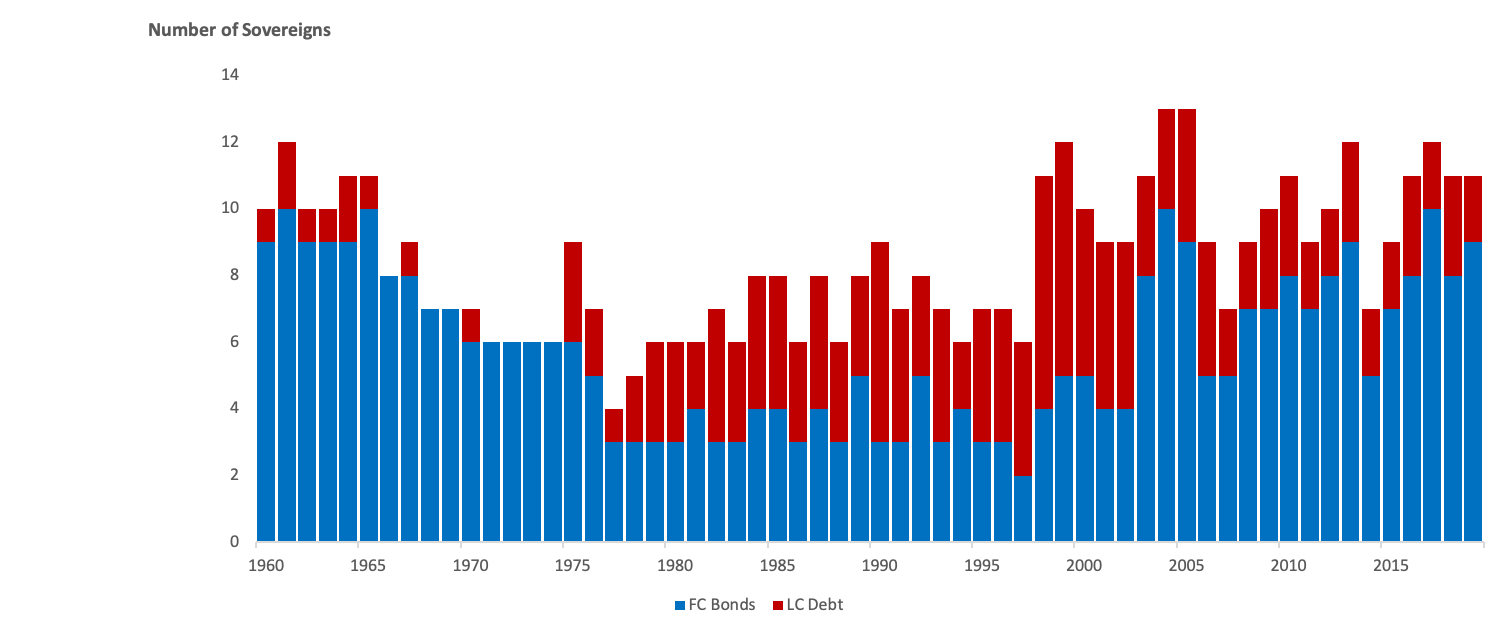
\includegraphics[width=0.8\textwidth,height=0.7\textheight]{../Figures/Slides/Defaults_FC_LC.png}
	\end{center}
	\begin{textblock*}{50mm}(23mm,83mm)
		\tiny Source: Beers, Jones and Walsh (2020).
	\end{textblock*}
\end{frame}
\note{A long-held view among some market participants is that governments rarely default on LC sovereign debt b/c they can print money}
\note{This figure shows you that
	Defaults on LC debt do occur and are more common than is usually thought.
	It is true that LC defaults are less frequent than FC defaults but the risk is there.
	This means that traditional decompositions of yield are not suitable for EM.
	
	LC default unlikely for countries with debt mainly in LC at long maturity.
	LC defaults have limited visibility 
	- governments rarely acknowledge them. 
	- impacted investors are mostly domestic residents with limited avenues of redress. Foreign investment in sovereign LC debt instruments (since 90s) increased awareness of more recent default cases.
	
	Examples of overt defaults in LC debt: Barbados (2018), Jamaica (2010, 2013), Nicaragua (2003, 2008), Argentina (2001), Turkey (1999) (earthquake, retroactively taxed LC debt), Russia (1998) after high inflation, Brazil 1990, Mexico 1982. El Salvador 2017, Cyprus 2013?}
\note{Debt denominated in LC has become an important source of funds for sovereigns and firms in EMs.}
\note{Foreign investor participation has increased from 10\% in 2008 to 25\% in 2019.}
%\note{in 2011, G20 launched initiative to support LC bond markets in EM.}

\begin{frame}
	\frametitle{Credit Risk in Local Currency Yields}
	\begin{center}
		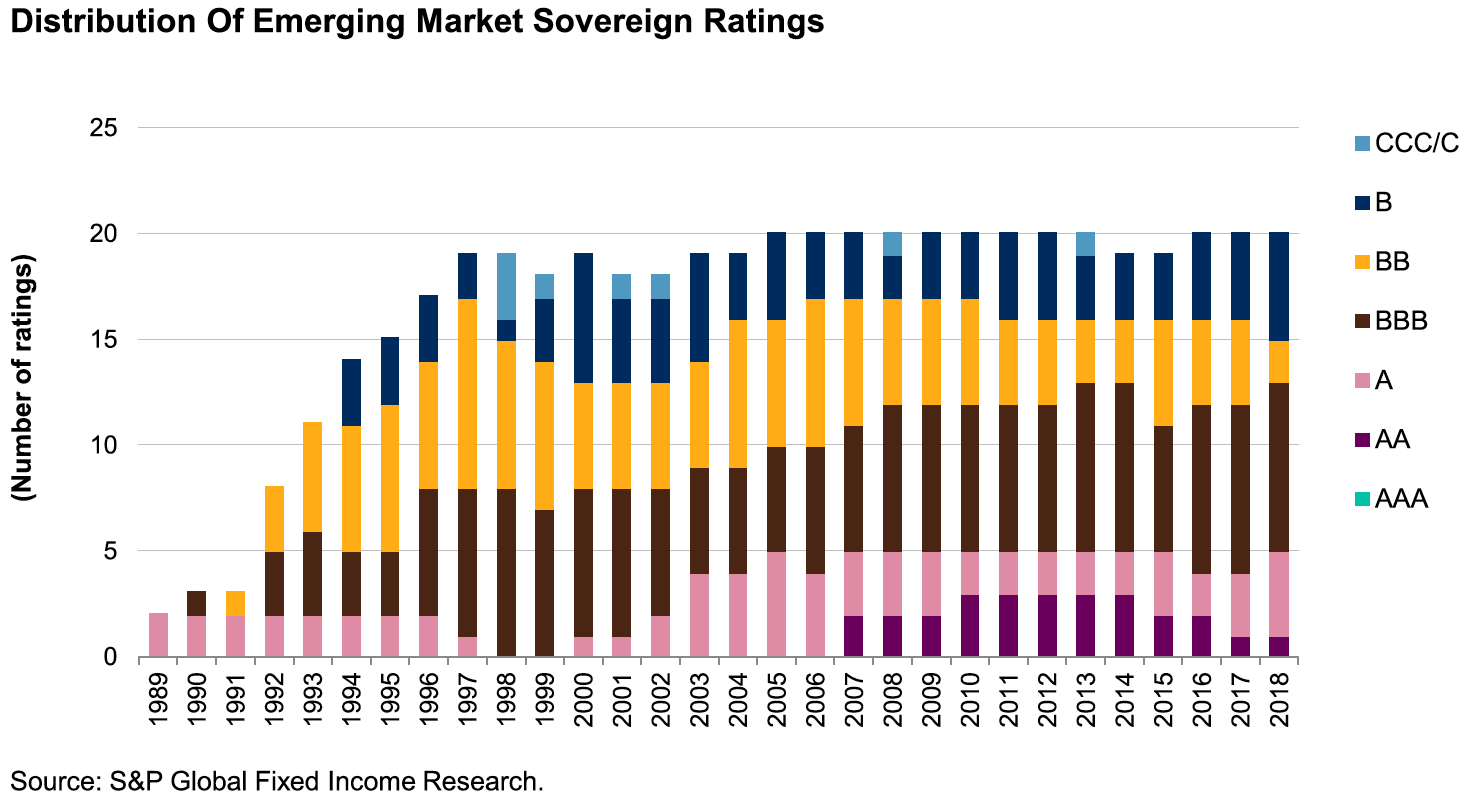
\includegraphics[width=0.8\textwidth,height=0.7\textheight]{../Figures/Slides/EM_LC_Ratings.png}
	\end{center}
\end{frame}
\note{Unlike AEs, credit risk in LC yields of EMs, even though they can print LC.}
\note{Since 1980 60+ default episodes under domestic law, bonds denominated in LC.}
\note{Number of domestic-law defaults has steadily increased over time.}
\note{Reflected in the credit ratings of LC bonds.}
\note{Credit risk broadly defined: (selective) default risk, currency convertibility risk, regulation risk, capital controls, jurisdiction risks, liquidity risk, sovereign restructurings.}
\note{EM ratings: Argentina, Brazil, China, Colombia, Egypt, Hungary, India, Indonesia, Lebanon, Malaysia, Mexico, Pakistan, Philippines, Poland, Qatar, Russia, Saudi Arabia, South Africa, Thailand, Turkey.}
\note{A bond is considered investment grade if its credit rating is BBB- or higher.}

\begin{frame}
	\frametitle{Research Questions}
	\begin{itemize}
		\item How to decompose sovereign yields of emerging markets (EM)?
		\item How does U.S. monetary policy transmit to EM yields?
		\begin{itemize}
			\item Does it influence expectations of future policy rates? 
			\item Does it affect the term premium?
			\item Does it impact creditworthiness?
		\end{itemize}
	\end{itemize}
%	\begin{textblock*}{3cm}(.85\textwidth,0.85\textheight)
%		\hyperlink{LitReview}{\beamergotobutton{Related Literature}}
%	\end{textblock*}
\end{frame}
\note{Quantify transmission channels of U.S. monetary policy to EM yields}
\note{Inform effective mitigation of undesired domestic impacts.}
%\note{Not only whether they comove but what drives the comovement.}
%\note{New perspective on the GFCy: financial conditions interrelated across countries.}
%\note{Better understanding of vulnerabilities in global financial system.}
%\note{These questions have barely received attention in the literature.}

%\begin{frame}[label=Contributions]
%	\frametitle{Contributions}
%	\begin{itemize}
%		\item Decomposition of EM sovereign yields accounting for credit risk
%		\item Quantify transmission channels of U.S. monetary policy to EM yields
%		\item Evidence on a yield curve channel of U.S. monetary policy
%	\end{itemize}
%	\begin{textblock*}{3cm}(.85\textwidth,0.85\textheight)
%		\hyperlink{LitReview}{\beamergotobutton{Related Literature}}
%	\end{textblock*}
%\end{frame}

\begin{frame}
\frametitle{EM Yield Decomposition}
\begin{center}
	\includegraphics[width=0.8\textwidth,height=0.75\textheight]{../Figures/Slides/Yield_Dcmp.png}
\end{center}
\end{frame}

\begin{frame}
	\frametitle{U.S. Monetary Policy Spillovers}
	\begin{enumerate}
		\item EM yields' response is economically significant, yet delayed over days
		\item All three components react
		\begin{itemize}
			\item Reassessment of policy rate expectations
			\item Repricing of interest and credit risks
		\end{itemize} 
		\item Unconventional measures limit EM monetary autonomy along the yield curve
	\end{enumerate}
\end{frame}

\begin{frame}[label=LitReview]
	\frametitle{Related Literature}
	\begin{itemize}
		\item Synthetic yields and covered interest rate parity deviations
		\vspace{-3mm}
		\item[] {\footnotesize Du-Schreger '16, Du-Im-Schreger '18, Du-Tepper-Verdelhan '18}
		\item Sovereign default in EM local currency bonds
		\vspace{-3mm}
		\item[] {\footnotesize Reinhart-Rogoff '11, Du-Schreger '16, Erce-Mallucci '18, Otonello-Pérez '19}
		\item Spillovers of U.S. monetary policy to EM yields
		\vspace{-3mm}
		\item[] {\footnotesize Hausman-Wongswan '11, Bowman-Londono-Sapriza '15, Curcuru-Kamin-Li-Rodríguez '18, Albagli-Ceballos-Claro-Romero '19, Adrian-Crump-Durham-Moench '19}
	\end{itemize}
%	\begin{textblock*}{3cm}(.87\textwidth,0.93\textheight)
%		\hyperlink{Contributions}{\beamerreturnbutton{Contributions}}
%	\end{textblock*}
\end{frame}
\note{Point out three things.}
\note{International comparison of bond yields has focused on AEs.}
\note{LC debt overlooked by the (theoretical and empirical) literature until recently.}

\begin{frame}
	\frametitle{Roadmap}
	\begin{itemize}
		\item Construction of yield curves
		\item Affine term structure model
		\item Decomposition of EM yields
		\item U.S. monetary policy spillovers
	\end{itemize}
\end{frame}



\begin{frame}
\begin{center}
	\huge \textcolor{yaleblue}{Construction of Yield Curves}
\end{center}
\end{frame}

\begin{frame}
	\frametitle{\textbf{Nominal} Yield Curves}
	\begin{itemize}
		\item Local currency (LC) nominal yield curves (\(\yLCnom\)) from:
		\begin{itemize}
			\item Bloomberg Fair Value (BFV) par yield curves \(\rightarrow\) Zero-coupon yield curves
		\end{itemize}
		\item \alert{Problem:} Credit risk embedded in LC nominal yields of EM % ($\yLCnom$)
		\item \alert{Approach:} Synthetic LC yields can be treated as \textit{free of credit risk}
		\begin{itemize}
			\item Swap U.S. Treasury yields into LC using \alert{currency derivatives}
			\item Why not CDS (credit default swaps)?
		\end{itemize}
	\end{itemize}
\end{frame}
\note{Sovereign debt of AEs is considered free of credit risk.}
%\note{Synthetic instead of nominal yields.}
\note{Under this approach, US YC used as a benchmark for all EMs.}
\note{CDS do not adequately characterize LC credit risk because defaults on LC bonds governed under domestic law are not triggers of CDS.}
%\note{Broad perspective on credit risk, i.e. not receiving promised payments: EMs can change the law + Suspension of currency convertibility + Capital controls + Actual default.}
%\note{BFV curves are par yield curves provided by Bloomberg on a daily basis for different maturities. To obtain the implied zero-coupon curves, the yields are converted into discount factors, which are then used to estimate the parameters of the Nelson-Siegel-Svensson model.}
%\note{CDS is a financial derivative that enable investors to swap credit risk.}

\begin{frame}[label=Synthetic]
	\frametitle{\textbf{Synthetic} Yield Curves}
	\vspace{-1cm}
	\begin{equation*} \label{eq:uLCsynt}
	\eqyLCsynt
\end{equation*}
	\vspace{-0.5cm}
	\begin{itemize}
		\item \(\yLCsynt\): \(\tnr\)-period zero-coupon \textit{synthetic} yield of a country in LC at time $t$
		\item \(\yUS\): \(\tnr\)-period zero-coupon yield of the U.S. in USD at time \(\idxt\)
		\item \(\fwdprm\): \(\tnr\)-period \alert{forward premium} from USD to LC at time \(\idxt\)
		\begin{itemize}
			\item Currency forwards (\(< 1\) year) and cross-currency swaps (\(\geq 1\) year)
		\end{itemize}
	\end{itemize}
%	\begin{textblock*}{3cm}(.92\textwidth,0.74\textheight)
%		\hyperlink{FwdPrm}{\beamergotobutton{FP}}
%	\end{textblock*}
\end{frame}
\note{FP compensates for the depreciation of the LC.}
\note{Notice that the nominal YC is not needed to get the synthetic YC.}
\note{Today I can lock in a risk-free investment in LC by 
	exchanging LC for USD, investing those USD in Tresuaries and enter into a forward contract agreeing to sell USD for LC in the future. Once I receive the payment from Treasuries, I exchange it back into LC.
	Don't need data on LC nominal yields to construct the synthetic yield.
	Spread b/w LCNOM and LCSYNT is the CRC
}

\begin{frame}[label=FwdPrm]
\frametitle{Forward Premium ($\fwdprm$)}
\begin{itemize}
	\item \alert{\(< 1\) Year}: Currency forwards
	\begin{center}
		\((forward_{t,\tnr} - spot_{t})/\tnr\)
	\end{center}
	\item \alert{\(\geq 1\) Year}: Fixed-for-fixed cross-currency swaps (XCS)
	\iftoggle{long}{\pause}{}
	\begin{itemize}
		\item Cross-currency basis swaps
		\item Interest rate swaps
	\end{itemize}
\end{itemize}
%\begin{textblock*}{3cm}(.86\textwidth,0.13\textheight)
%	\hyperlink{Synthetic}{\beamergotobutton{Synthetic Yields}}
%\end{textblock*}
\end{frame}
\note{Currency forwards liquid up to 1Y.}
\note{Fixed-for-fixed XCS not directly traded in the market but they can be constructed.}
\note{CCS and IRS are liquid and collateralized. Bilateral counterparty risk is small.}

\begin{frame}[label=DevCIP]
\frametitle{Deviations from CIP (Covered Interest Parity)}
\vspace{-1cm}
\[\eqCIPdevQ\]
\vspace{-1.2cm}
\begin{itemize}
	\item Measure of:
	\begin{itemize}
		\item Sovereign credit risk for EM \citep{DuSchreger:2016JoF} % (Du-Schreger '16)
		\item Convenience yield for advanced countries \citep*{DuImSchreger:2018JIE} % (Du-Im-Schreger '18)
		\item Financial market frictions for banks \citep*{DuTepperVerdelhan:2018} % (Du-Tepper-Verdelhan '18)
	\end{itemize}
\end{itemize}
\end{frame}
\note{Diff b/w nominal and synthetic measures CIP deviations in government yields.}
\note{Correlation b/w CIP dev and CDS is high for EMs but not for AEs.}


\section{Data}

\begin{frame}
\frametitle{Data}
\begin{itemize}
	\item EM (15) countries:
	\item[] {\scriptsize BRL, COP, HUF, IDR, ILS, KRW, MYR, MXN, PEN, PHP, PLN, RUB, THB, TRY, ZAR}
%	\item[] {\scriptsize Brazil, Colombia, Hungary, Indonesia, Israel, Korea, Malaysia, Mexico, Peru, Philippines, Poland, Russia, Thailand, Turkey, South Africa}
%	\begin{itemize}
%		\item \scriptsize \alert{10 AEs}: AUD, CAD, CHF, DKK, EUR, GBP, JPY, NOK, NZD, SEK
%	\end{itemize}
	\iftoggle{struct}{\item<2->}{\item} Daily data from \(\sim\)Jan-2000 to Jan-2019
	\iftoggle{struct}{\item<3->}{\item} Maturities (in years): 0.25, 0.5, 1, 2, \ldots, 10
	\iftoggle{struct}{\item<4->}{\item} Sources:
	\begin{itemize}
		\iftoggle{struct}{\item<5->}{\item} $\yUS$: CRSP Risk-Free Rates Series, \citet*{GSW:2007}
		\vspace{-0.1cm}
		\iftoggle{struct}{\item<6->}{\item} $\fwdprm$: Bloomberg $+$ Datastream
	\end{itemize}
\end{itemize}
\end{frame}
\note{Currency identifier for each country is shown.}
\note{Results are compared against those obtained for 10 AEs.}
\note{Starting dates vary by country.}
\note{At least 10 years of data}
\note{Longer series desirable to pin down TP since unobserved. But >10Y reasonable.}
\note{U.S. yield curve from GSW database.}
\note{Treasury securities with less than one year to maturity are less actively traded than longer-maturity ones. CRSP data is thought to be more robust at the short end.}
%\note{Reasons for use monthly: VAR is a good approximation for monthly, adequate frequency if want to use macro data.}
%\note{Consensus Economics provides long-horizon forecasts for consumer inflation and real GDP growth but not for policy rates.}

\begin{frame}
\begin{center}
	\huge \textcolor{yaleblue}{Affine Term Structure Model}
\end{center}
\end{frame}

\section{Methodology}

\begin{frame}[label=ATSM]
	\frametitle{Model Overview}
	\begin{itemize}
		\item Standard discrete-time nominal affine term structure model \(+\) Survey data
		\item A set of pricing factors drives the dynamics of the term structure
		\item No-arbitrage restrictions ensure consistency in cross section and time series %of yields
		\item Yields are affine functions of the pricing factors
		\item Assumption: Default-free bonds \(\rightarrow\) Synthetic yields (\(\yLCsynt\))
	\end{itemize}
%	\begin{textblock*}{3cm}(.89\textwidth,0.82\textheight)
%		\hyperlink{Qdynamics}{\beamergotobutton{Q Dynamics}}
%	\end{textblock*}
%	\begin{textblock*}{3cm}(.89\textwidth,0.88\textheight)
%		\hyperlink{Pdynamics}{\beamergotobutton{P Dynamics}}
%	\end{textblock*}
%	\begin{textblock*}{3cm}(.89\textwidth,0.94\textheight)
%		\hyperlink{Components}{\beamergotobutton{Decomposition}}
%	\end{textblock*}
\end{frame}
\note{ATSM standard tool to estimate dynamics of risk-free \alert{nominal} yield curves.}
\note{Coefficients: functions of the bond maturity and parameters of the model.}
\note{Once parameters estimated, decompose yields into expected short rate and TP.}
\note{Assumption yields are risk-free.}
\note{Decomposition into: YP and TP.}
%\note{The coefficients are functions of the maturity of the bond and the coefficients that determine the stochastic processes that drive the state variables.}

\begin{frame}[label=Qdynamics]
\frametitle{Dynamics Under \(\Qmeasure\) Measure}
\begin{itemize}
	\item Pricing factors under risk-neutral measure \(\Qmeasure\)
	\begin{equation*} \label{eq:uXvarsQ}
	\eqXvarsFwdQ 
\end{equation*}
	\item Dynamics of one-period interest rate
	\begin{equation*} \label{eq:uShortRate}
	\eqshortrate 
\end{equation*}
	\item Fitted yields and loadings
	\begin{equation*}
	\eqyZeroQ
\end{equation*}

%	\yZeroQ = \affineA^{\Qmeasure} + \affineB^{\Qmeasure} \Xvars
\end{itemize}
%\begin{textblock*}{3cm}(.92\textwidth,0.13\textheight)
%	\hyperlink{ATSM}{\beamergotobutton{Overview}}
%\end{textblock*}
\end{frame}

\begin{frame}[label=Pdynamics]
\frametitle{Dynamics Under \(\Pmeasure\) Measure}
\begin{itemize}
\item Stochastic discount factor
\begin{equation*} \label{eq:uSDF}
	\eqSDF 
\end{equation*}
\item Market prices of risk
\begin{equation*} \label{eq:uRiskprice}
	\eqriskprice 
\end{equation*}
\item Pricing factors under physical measure \(\Pmeasure\)
\begin{equation*} \label{eq:uXvarsP}
	\eqXvarsFwdP
\end{equation*}
\end{itemize}
%\begin{textblock*}{3cm}(.92\textwidth,0.13\textheight)
%\hyperlink{ATSM}{\beamergotobutton{Overview}}
%\end{textblock*}
\end{frame}

\begin{frame}[label=Components]
\frametitle{EM Yield Decomposition}
\begin{itemize}
\item Future expected short rate as if investors were risk-neutral (\(\lambdazero = \lambdaone = 0\))
\begin{equation*}
	\yZeroP = \affineAP + \affineBP \Xvars,
	%\yZeroP = - \frac{\affineA}{\tnr} - \frac{\affineB}{\tnr} \Xvars = \affineA^{\Pmeasure} + \affineB^{\Pmeasure} \Xvars,
\end{equation*}
\(\affineAP = - \frac{1}{\tnr} \affineA\), \(\affineBP = - \frac{1}{\tnr} \affineB\), \(\affineA = A(\deltazero, \deltaone, \XmuP, \XPhiP, \XSigma, \tnr)\) and \(\affineB = \mathcal{B}(\deltaone, \XPhiP, \tnr)\)
\item Term premium
\begin{equation*} \label{eq:uTPatsm}
	\termprm = \yZeroQ - \yZeroP.
\end{equation*}
\item Credit risk compensation
\[\CIPdev = \yLCnom - \yZeroQ\]
\end{itemize}
%\begin{textblock*}{3cm}(.92\textwidth,0.13\textheight)
%\hyperlink{ATSM}{\beamergotobutton{Overview}}
%\end{textblock*}
\end{frame}
\note{Synthetic curve better aligns with the risk-free assumption.}
\note{ATSM for synthetic allows to decompose nominal into 3 parts.}


\begin{frame}
	\frametitle{Weak Identification}
	\begin{itemize}
		\item Bond yields are persistent $\rightarrow$ Small sample bias \citep{KimOrphanides:2012}
		\begin{itemize}
%			\item Overestimates stability of expected path of short rate
			\item Most variability attributed to fluctuations in term premium
		\end{itemize}
	\item Solutions: survey data, parameter restrictions, bias-corrected estimators
	\item \alert{Surveys} provide robust decompositions of yields \citep{Guimaraes:2014}
	\begin{itemize}
		\item Important for EM due to small sample sizes
	\end{itemize}
	\end{itemize}
\end{frame}
\note{Overestimates stability of expected path of short rate}
\note{Estimation requires long time series}
\note{Only ZC bond yields are needed to estimate ATSM parameters.}
\note{However, TP is an unobserved variable.}
\note{Uses of surveys: (1) model-free TP estimate. (2) supplement in ATSMestimation.}
%\note{Surveys are an effective solution to obtain robust decompositions of the yield curve \citep{Guimaraes:2014} 

\begin{frame}[label=SCBP]
\frametitle{Survey Data}
\begin{itemize}
	\item No data on long-term forecasts for the short rate in EM
	\item Implied value from existing data on long-term forecasts
	\begin{itemize}
		\item EM inflation expectations from Consensus Economics (twice a year)
		\item Implied U.S real rate from Survey of Professional Forecasters
		\begin{itemize}
			\item T-bill rate, CPI inflation
			\item Compared against TIPS yields
		\end{itemize}
	\end{itemize}
\end{itemize}
%\begin{textblock*}{3cm}(.87\textwidth,0.47\textheight)
%	\hyperlink{SvyAugModel}{\beamergotobutton{Implied Forecast}}
%\end{textblock*}
\end{frame}
\note{Rely on the SEO assumption -> Fisher equation.}
\note{Use them in survey augmented model.}
\note{Data available twice a year.}


\begin{frame}[label=SvyAugModel]
\frametitle{Survey-Augmented Model}
\begin{itemize}
	\item Implied forecast for the short rate in EM
	\begin{equation*} \label{eq:uRrt}
	\eqrrt
\end{equation*}
	\item Expected average short rate under \(\Pmeasure\)
	\begin{equation*}
	\yZeroE = \frac{1}{\tnr} \ExpP \left[ \sum_{j=0} ^{\tnr-1} \srate_{\idxt+j} \right] = \affineAe + \affineBe \Xvars,
\end{equation*}
	\item Forward rate from \(\tnr\) to \(\tnrfwd\) periods hence
	\begin{equation*}
	\yZeroEfwd = \affineAeFwd + \affineBeFwd \Xvars.
\end{equation*}
\end{itemize}
%\begin{textblock*}{3cm}(.9\textwidth,0.14\textheight)
%	\hyperlink{SCBP}{\beamergotobutton{Survey Data}}
%\end{textblock*}
\end{frame}

\begin{frame}
\frametitle{Estimation}
\begin{itemize}
%	\item Use \cite*{JSZ:2011} normalization of the model %: \(\Pmeasure \perp \Qmeasure\) % likelihood functions
	\item Estimate parameters by MLE
	\begin{itemize}
		\item \cite*{JSZ:2011} normalization of the model
	\end{itemize}
%	\item Estimate \(\Pmeasure\) parameters by OLS
%	\item Estimate \(\Qmeasure\) parameters by MLE
	\item Estimate survey-augmented model by Kalman filter (missing data)
	\begin{itemize}
		\item Surveys viewed as `noisy' measures of expectations
	\end{itemize}
	\item Compute standard errors by delta method
	\item Estimate daily pricing factors
\end{itemize}
\end{frame}
\note{End-of-month data}

\section{Decomposition}

\begin{frame}
\begin{center}
	\huge \textcolor{yaleblue}{Decomposition of EM Yields}
\end{center}
\end{frame}


\begin{frame}[label=ModelFit]
%	\frametitle{Model Fit}
	\begin{center}							% center the figure inside the minipage
		\includegraphics[trim={0cm 0cm 0cm 0cm},clip,height=0.86\textheight,width=\linewidth]{../Figures/Estimation/s_ylds_bsl_yQ.eps} \\
	\end{center}
\end{frame}

\begin{frame}[label=YldDcmp]
%	\frametitle{Decomposition of EM Nominal Yields}
	\begin{center}							% center the figure inside the minipage
		\includegraphics[trim={0cm 0cm 0cm 0cm},clip,height=0.86\textheight,width=\linewidth]{../Figures/Estimation/ny_dcmp.eps} \\
	\end{center}
	\begin{textblock*}{5cm}(.11\textwidth,0.05\textheight)
		\hyperlink{yPscbp}{\beamergotobutton{Future Expected Short Rate}}
	\end{textblock*}
	\begin{textblock*}{3cm}(.44\textwidth,0.05\textheight)
		\hyperlink{tpCI}{\beamergotobutton{Term Premium}}
	\end{textblock*}
	\begin{textblock*}{5cm}(.66\textwidth,0.05\textheight)
		\hyperlink{crcCI}{\beamergotobutton{Credit Risk Compensation}}
	\end{textblock*}
\end{frame}
\note{Dynamics of TP and LCCS important in EM bond yields.}
\note{EM TP estimates assessed against stylized facts for USTP.}
\note{Events: GR, TT, US election, 2009 QE1.}
\note{TP decline due to: international investors, US UMP.}
%\note{USTP increased around the onset of the Great Recession (September 2008), the taper tantrum (June 2013), and the 2016 U.S. presidential election (November 2016), while it declined after the first unexpected announcement of the QE program by the Fed (March 2009).}
%\note{Common explanations for the decline in the USTP include an increased demand of U.S. assets by global investors and the effects of the UMP of the Fed.}
%\note{Explanation for change in sign (Campbell, Sunderam \& Viceira (2016)): TP < 0 is explained by the flip in the sign of the correlation between stocks and bonds -bonds hedge stocks-.}


\begin{frame}[label=tpUCSV]
\frametitle{Term Premium and Inflation Uncertainty}
\begin{itemize}
	\item Compensates investors for bearing inflation uncertainty \citep{Wright:2011}
	%In advanced countries related to inflation uncertainty \citep{Wright:2011} % in advanced countries
	\item EM inflation higher and more volatile \citep{HaKoseOhnsorge:2019}
	\item Is inflation uncertainty more relevant to term premia in EM?
\end{itemize}
\end{frame}

\begin{frame}
\frametitle{EM Term Premium and Inflation Uncertainty}
%	\setbeamercolor{background canvas}{bg=}
%	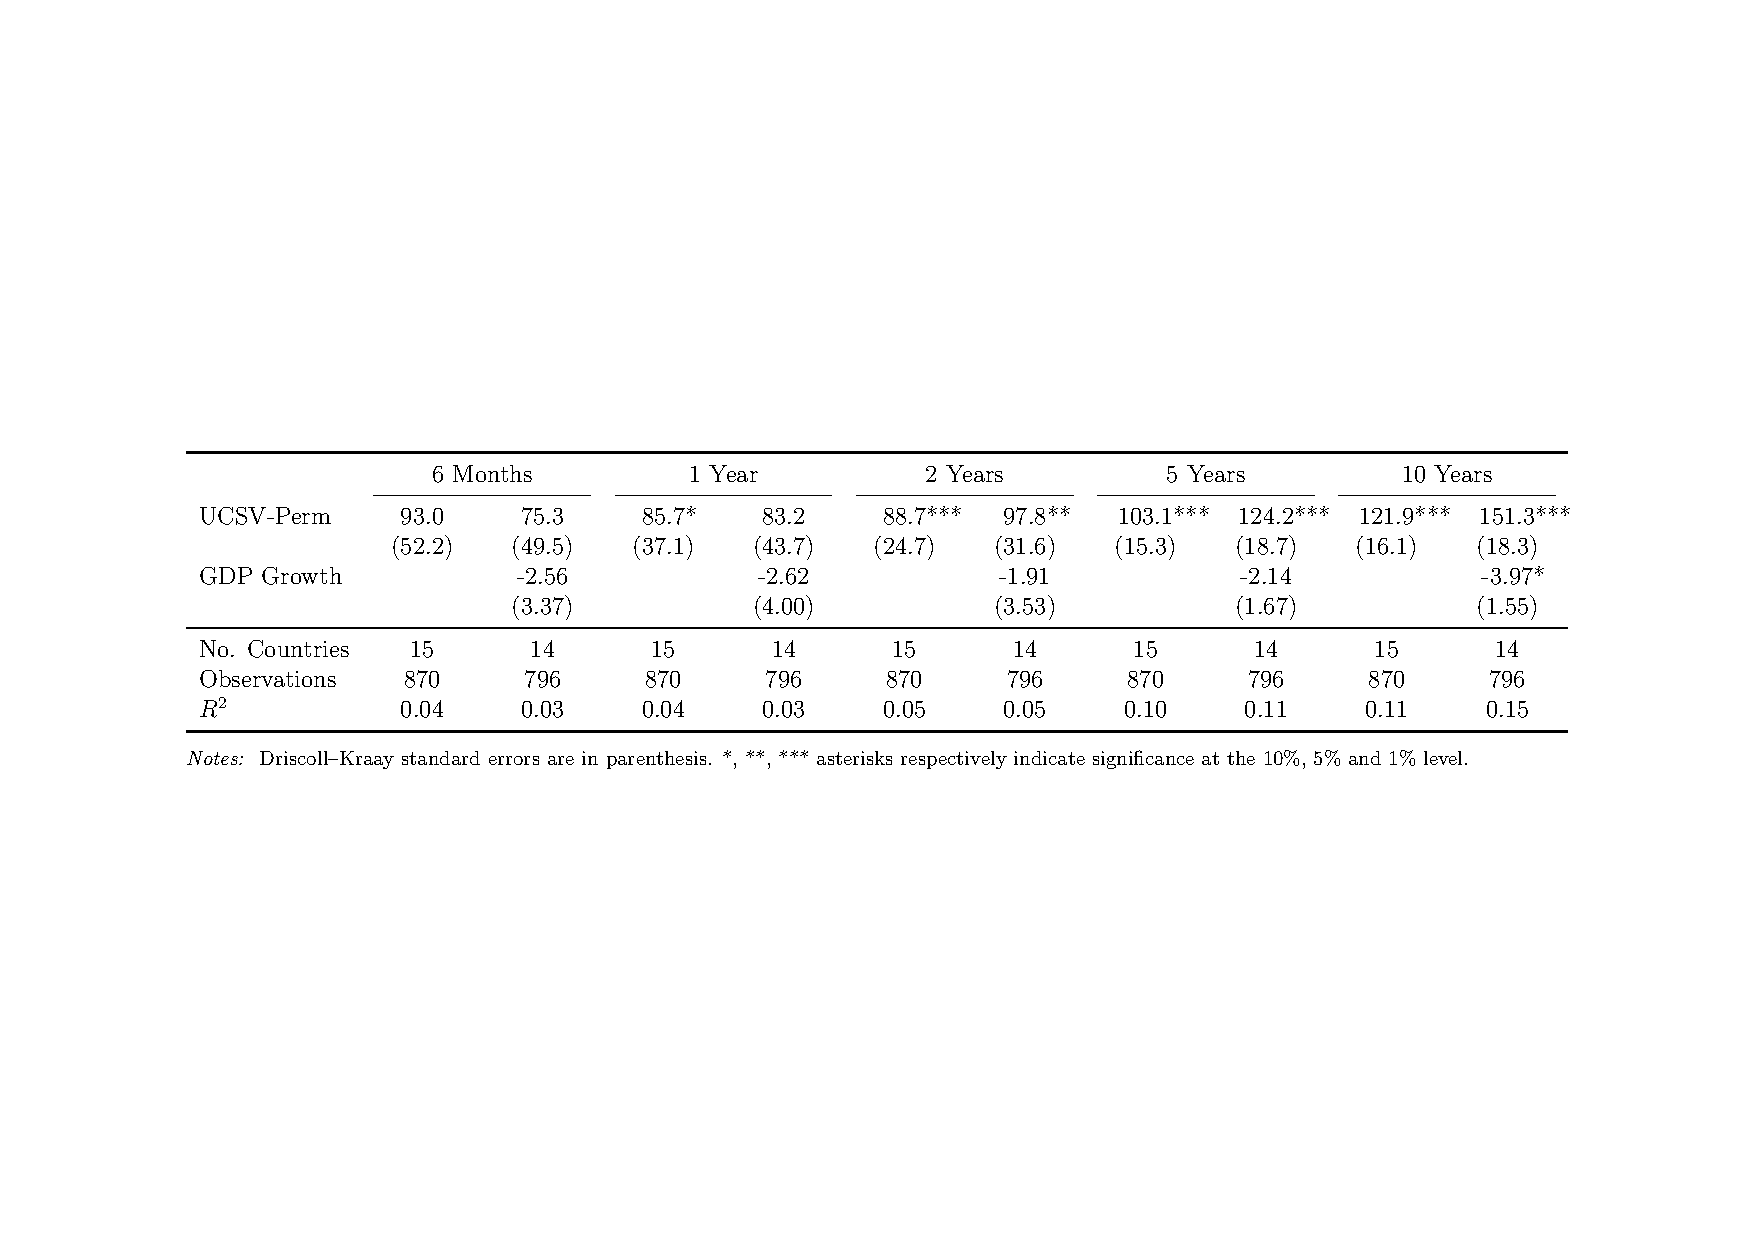
\includepdf[pages={1}]{../Tables/tpucsv.pdf}
\vspace{-0.8cm}
\begin{figure}[!htbp]
\begin{center} % trim removes: left, down, right, top
	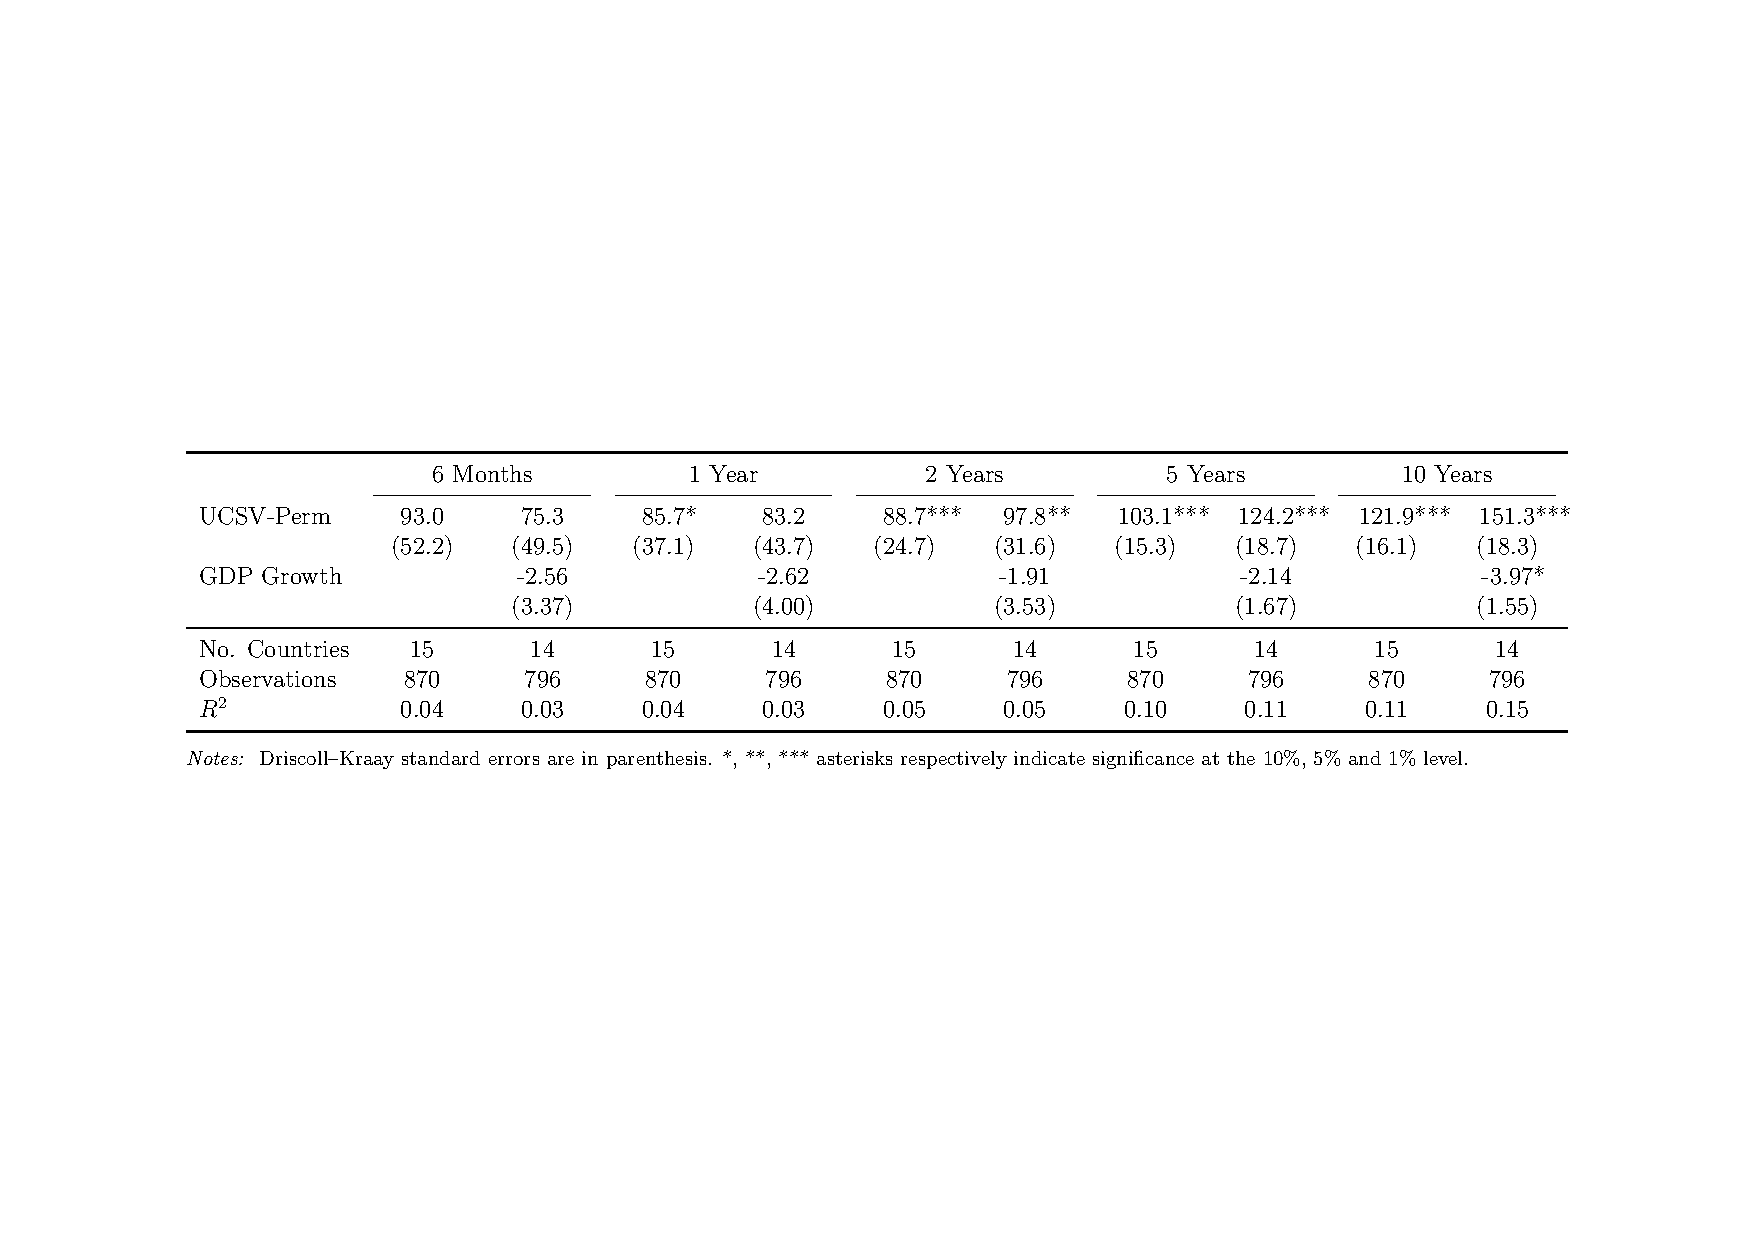
\includegraphics[trim={2cm 6cm 2cm 6.5cm},clip, width=1\textwidth,height=0.7\textheight]{../Tables/tpucsv.pdf}
	\par\end{center}
\end{figure}
\end{frame}


\section{Spillovers}

\begin{frame}
	\begin{center}
		\huge \textcolor{yaleblue}{U.S. Monetary Policy Spillovers}
	\end{center}
\end{frame}

\begin{frame}
	\frametitle{The Yield Curve Channel}
	\begin{itemize}
		\item Long-term yields highly correlated, influenced by global forces
		\item Unconventional monetary policies abroad affect EM long-term yields
		\begin{itemize}
			\item Via the term premium \citep{Turner:2014}
		\end{itemize}
		\item EM monetary autonomy:
		\begin{itemize}
			\item Declines along the yield curve \citep{Obstfeld:2015}
			\item Limited also at the short end \citep{Kalemli-Ozcan:2019}
		\end{itemize}
	\end{itemize}
\end{frame}

\begin{frame}
\frametitle{Implications of the Yield Curve Channel}
\begin{itemize}
	\item Do long-term EM yields comove more than short-term ones?
	\begin{itemize}
		\item \cite{DieboldYilmaz:2014} connectedness index
	\end{itemize}
	\item Direct relationships
	\begin{itemize}
		\item Term premium in the U.S. and in EM
		\item Expected future short rates in the U.S. and in EM
	\end{itemize}
	\item Cross relationships at the short end
	\begin{itemize}
		\item U.S. term premium and expected future short rates in EM
	\end{itemize}
\end{itemize}
\end{frame}
\note{Cross effect at 2Y maturity.}

\begin{frame}
	\frametitle{Comovement of EM Yields}
	\begin{figure}[!htbp]
		\begin{center} % trim removes: left, down, right, top
			\includegraphics[trim={0cm 0cm 0cm 0cm},clip,height=0.7\textheight,width=0.85\linewidth]{../Figures/Estimation/dy_index_dn_data.eps}
			\par\end{center}
	\end{figure}
	\begin{textblock*}{70mm}(50mm,83mm)
		\tiny \cite{DieboldYilmaz:2014} connectedness index
	\end{textblock*}
\end{frame}

\begin{frame}
\frametitle{Is There A Yield Curve Channel?}
%\begin{itemize}
%	\item Panel regression:
	\vspace{-1cm}
			\begin{equation*} \label{eq:uPanelDCMP}
	\eqpanelTPreg
\end{equation*}
	\vspace{-1cm}
	\begin{itemize}
		\item \(\yld_{\idxspnl}\): nominal yields and their three components
		\item \(\alpha_{i}\): country fixed effects
		\item \(z_{it}\): vector of regressors
		\begin{itemize}
			\item U.S. yield curve decomposition \citep{KimWright:2005}
			\item Global drivers: Vix, EPU index, Hamilton index
			\item Domestic drivers: Policy rate, inflation, unemployment, exchange rate %(LC per USD)
		\end{itemize}
	\end{itemize}
%\end{itemize}
\end{frame}
\note{Country FE allow for the possibility that country-specific factors that may affect TP are also correlated with the controls.}

\begin{frame}
%	\frametitle{EM Term Premium and Inflation Uncertainty}
\vspace{-0.8cm}
	\begin{figure}[!htbp]
		\begin{center} % trim removes: left, down, right, top
			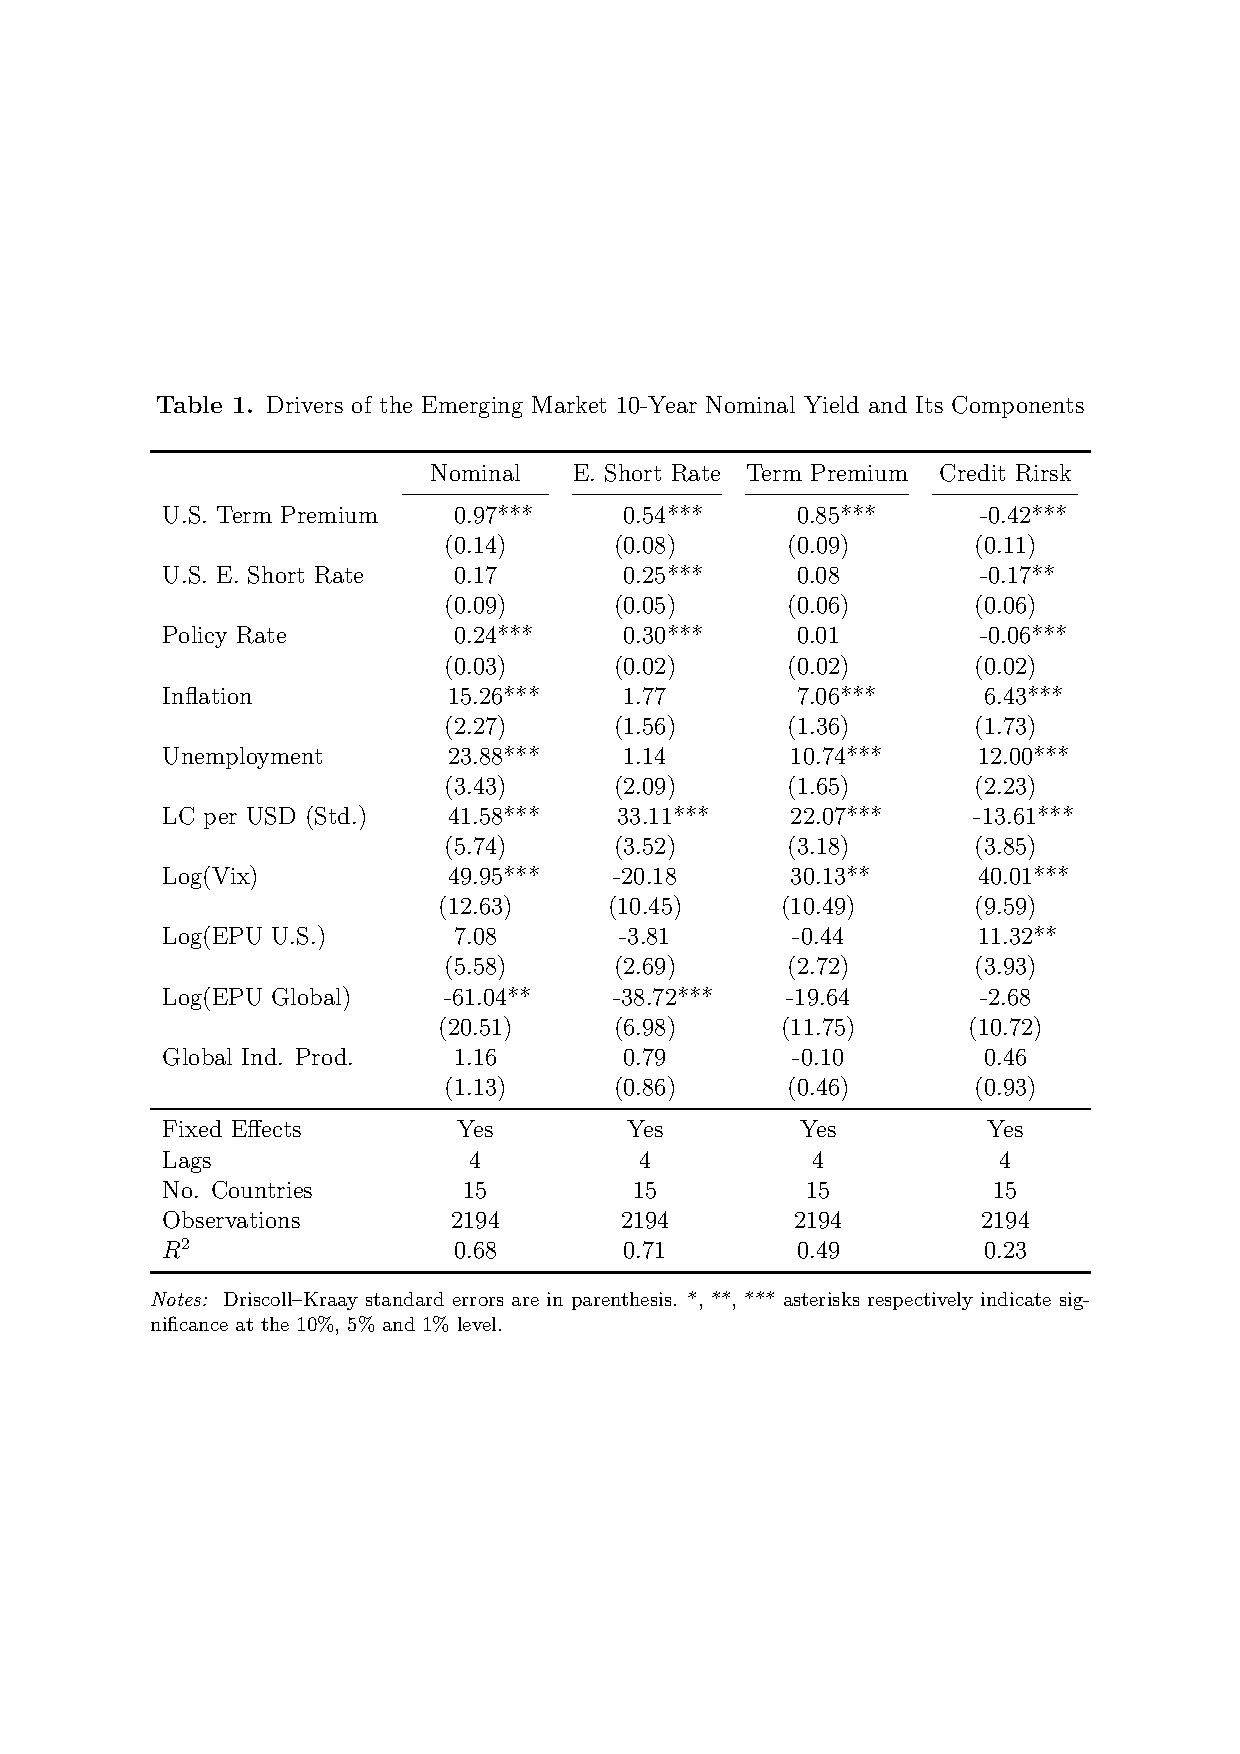
\includegraphics[trim={2cm 7.1cm 2cm 5cm},clip, width=0.85\textwidth,height=1\textheight]{../Tables/ycdcmp10y.pdf}
			\par\end{center}
	\end{figure}
\end{frame}

%\begin{frame}
%%	\frametitle{EM Term Premium and Inflation Uncertainty}
%	\vspace{-0.8cm}
%	\begin{center}
%	\begin{tikzpicture}
%	\node (table) at (0,0)
%	{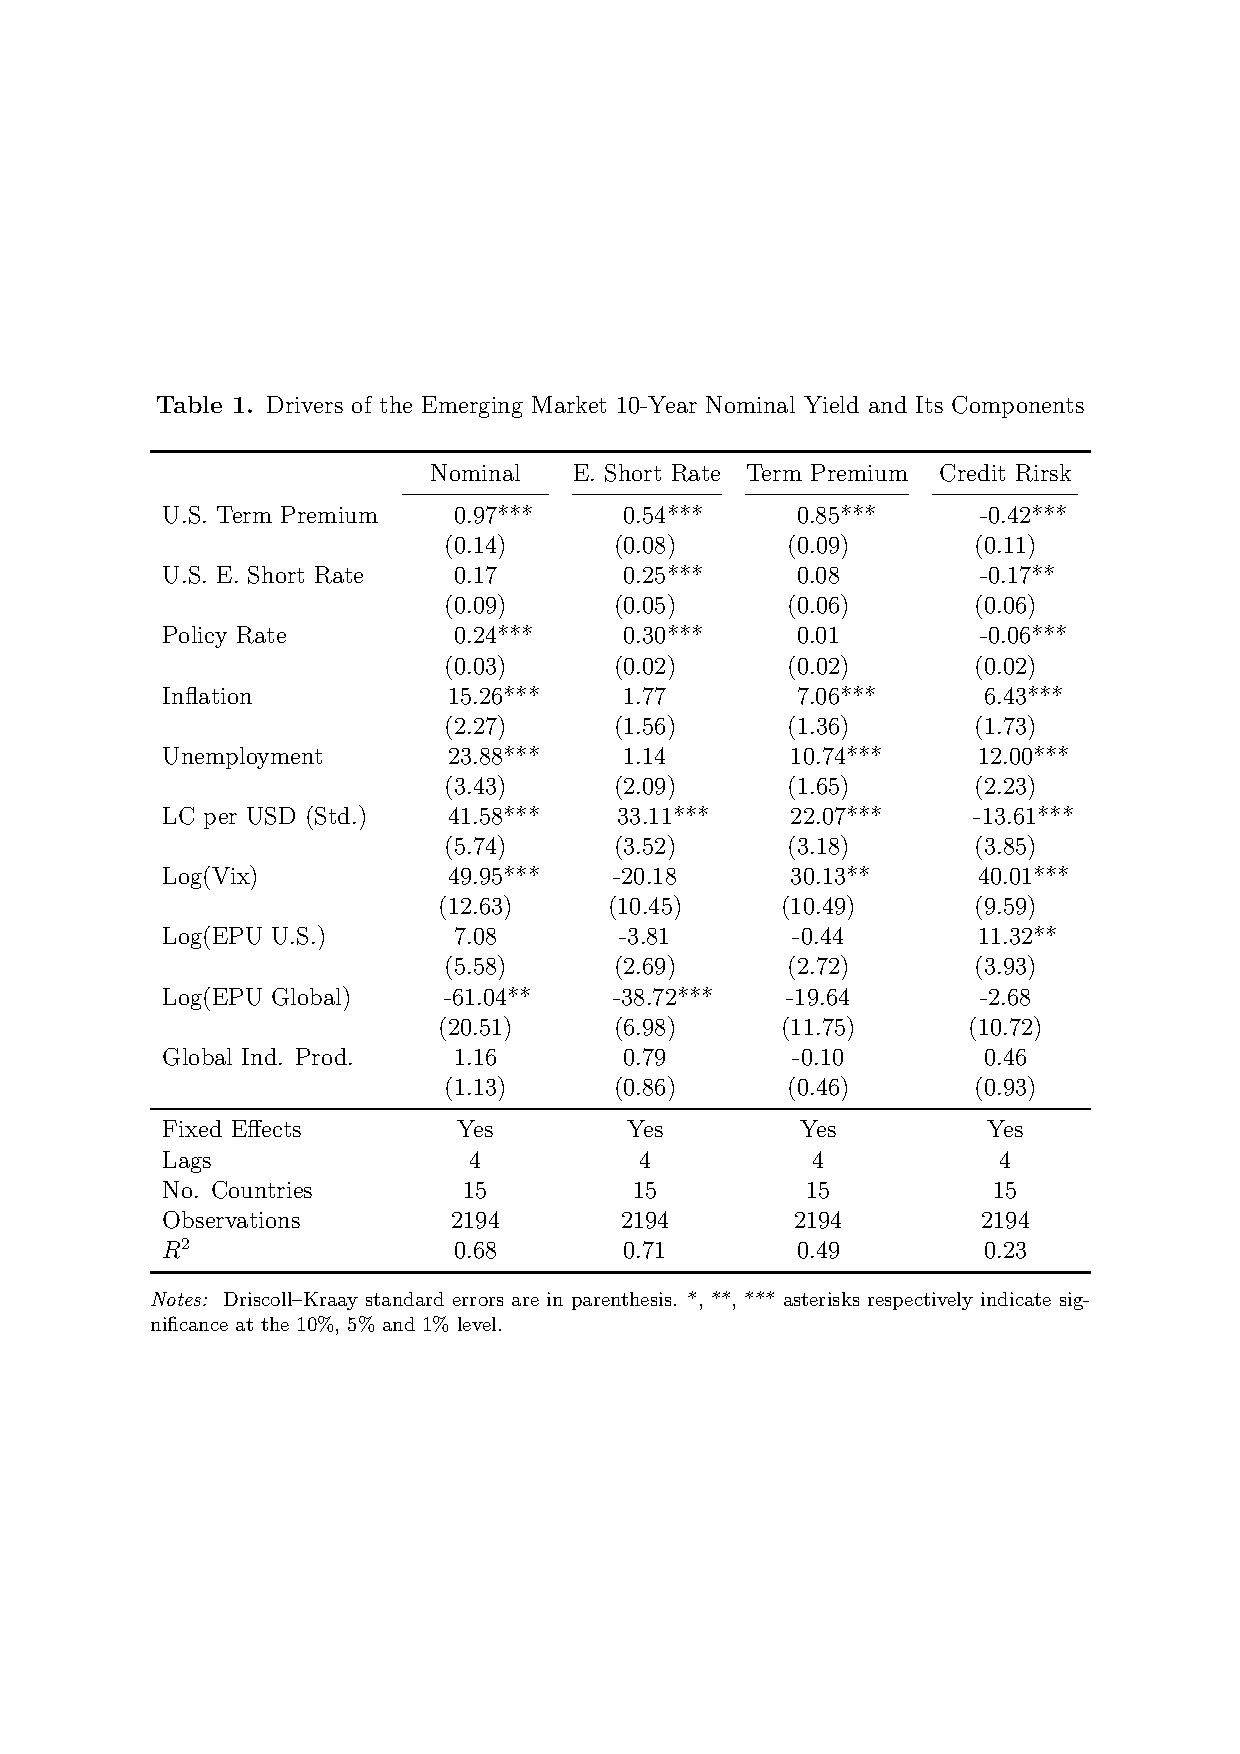
\includegraphics[trim={2cm 7.1cm 2cm 5cm},clip,height=1\textheight,width=0.85\textwidth]{../Tables/ycdcmp10y.pdf}};
%	%\draw[step=1cm,gray,very thin] (-4,-4) grid (6,6);
%	\draw[red,thick] (-6,1.6) rectangle (6,2.6);
%	\end{tikzpicture}
%	\end{center}
%\end{frame}
%\note{Confirms that external conditions impact domestic bond markets.}
%\note{US MP has effect not through FFR directly but via USTP.}
%\note{Effect of the domestic variables in line with findings for AEs.}
%\note{Higher TP during recessions: high UNE, low IP. Evidence of EM TP countercyclical.}
%\note{INF erodes value of nominal bonds: in periods of rising INF demand a higher TP.}
%\note{Higher TP due to FX depreciation in line with risk-taking channel of FX.
%	Currency depreciation tightens financial conditions, higher sovereign bond spreads.}
%\note{Main broad message at 10 years. Big difference: FFR more negative when there is no USTP and disappears when USTP.}
%\note{Effect of the domestic variables in line with findings for AEs. 
%	Investors demand a higher term premium during recessions, when the unemployment rate increases. This shows evidence of a countercyclical behavior of the TP in EMs.
%	The positive effect of inflation on the TP conforms with the idea that inflation erodes the value of nominal bonds and so in periods of rising inflation investors demand a higher TP.}
%\note{A depreciation of the LC is associated with an increase in the TP. This seems counterintuitive since EMs are usually commodity exporters so it appears to contradict the standard trade-channel effect. 
%	However, it is in line with the risk-taking channel of exchange rates found by \cite{HofmannShimShin:2017}, according to which currency depreciation is associated with tighter financial conditions and increased sovereign bond spreads.}


\begin{frame}
%	\frametitle{EM Term Premium and Inflation Uncertainty}
\vspace{-0.8cm}
\begin{figure}[!htbp]
	\begin{center} % trim removes: left, down, right, top
		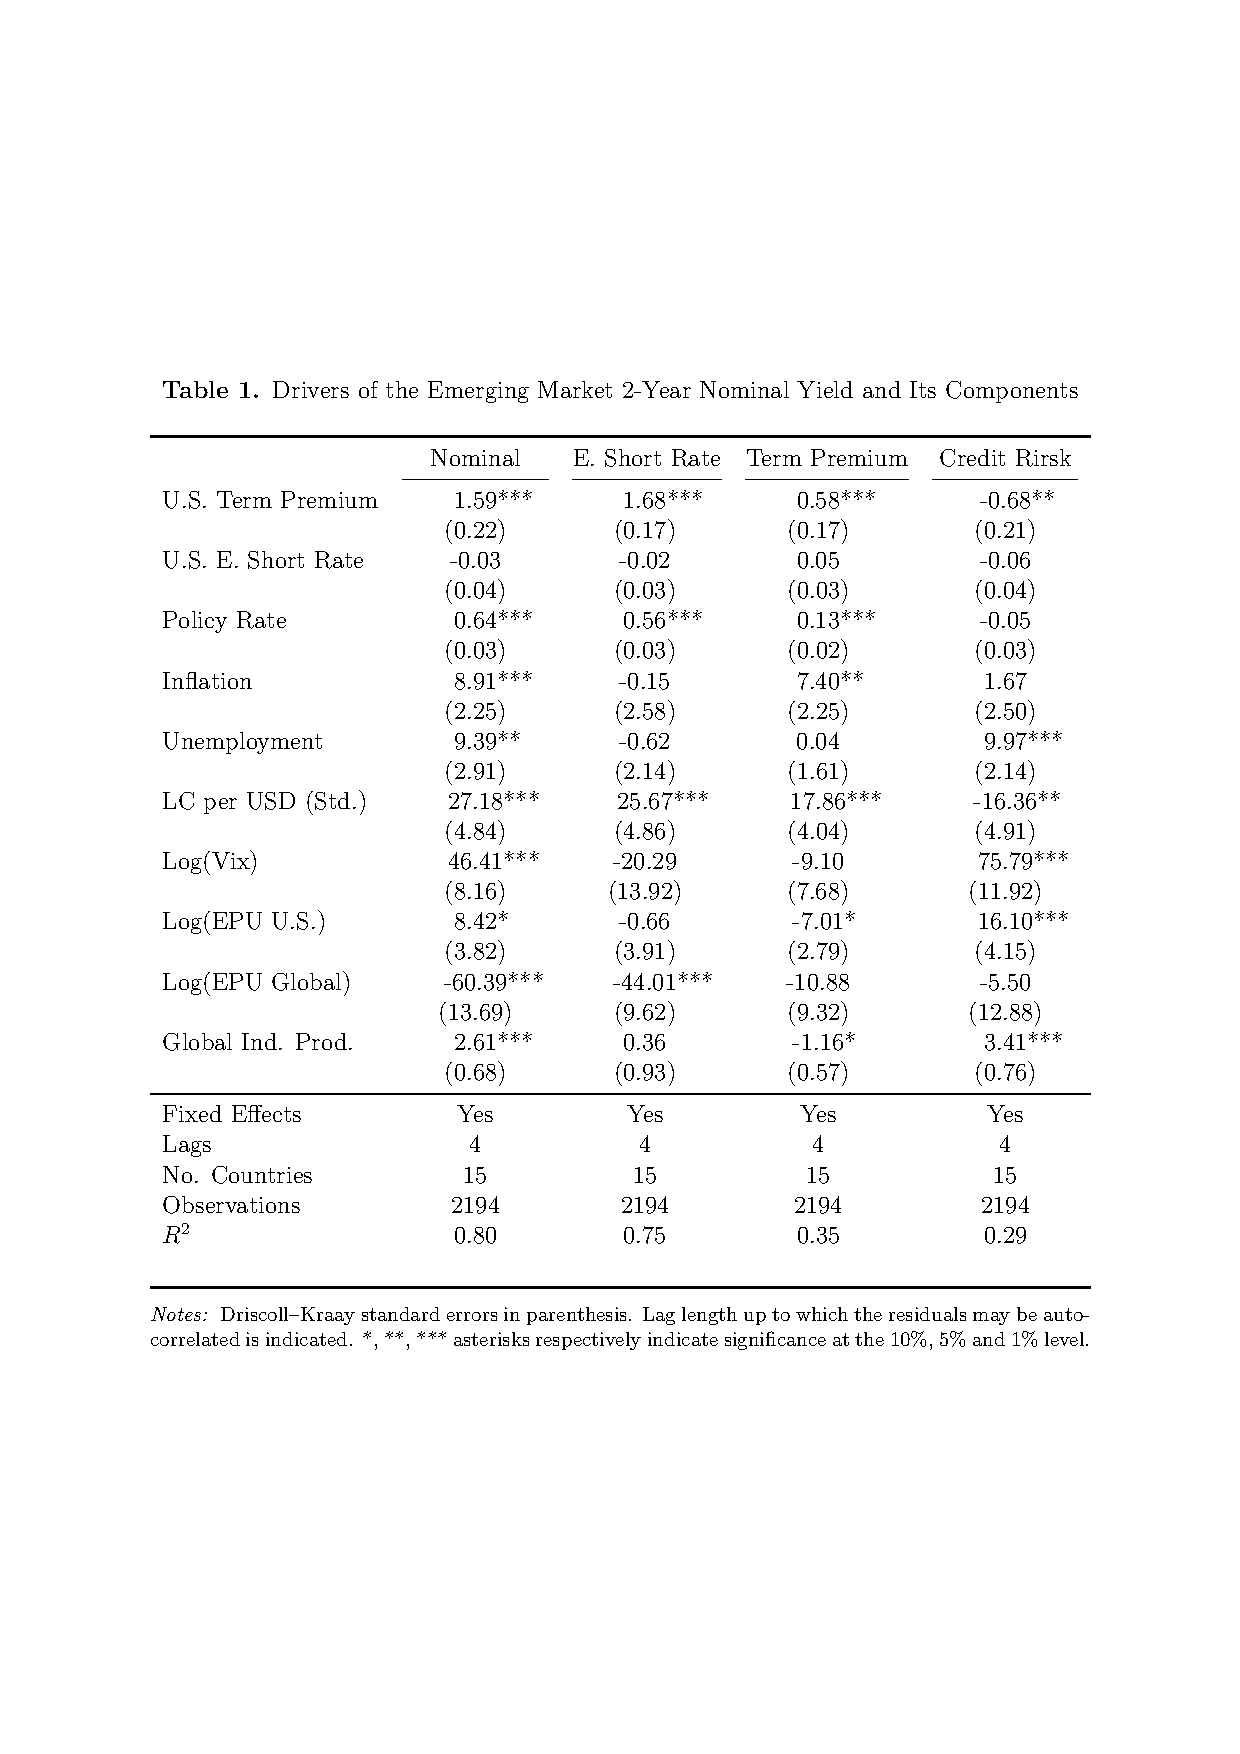
\includegraphics[trim={2cm 7.1cm 2cm 5cm},clip, width=0.85\textwidth,height=1\textheight]{../Tables/ycdcmp2y.pdf}
		\par\end{center}
\end{figure}
\end{frame}

%\begin{frame}
%%	\frametitle{EM Term Premium and Inflation Uncertainty}
%\vspace{-0.8cm}
%\begin{center}
%	\begin{tikzpicture}
%	\node (table) at (0,0)
%	{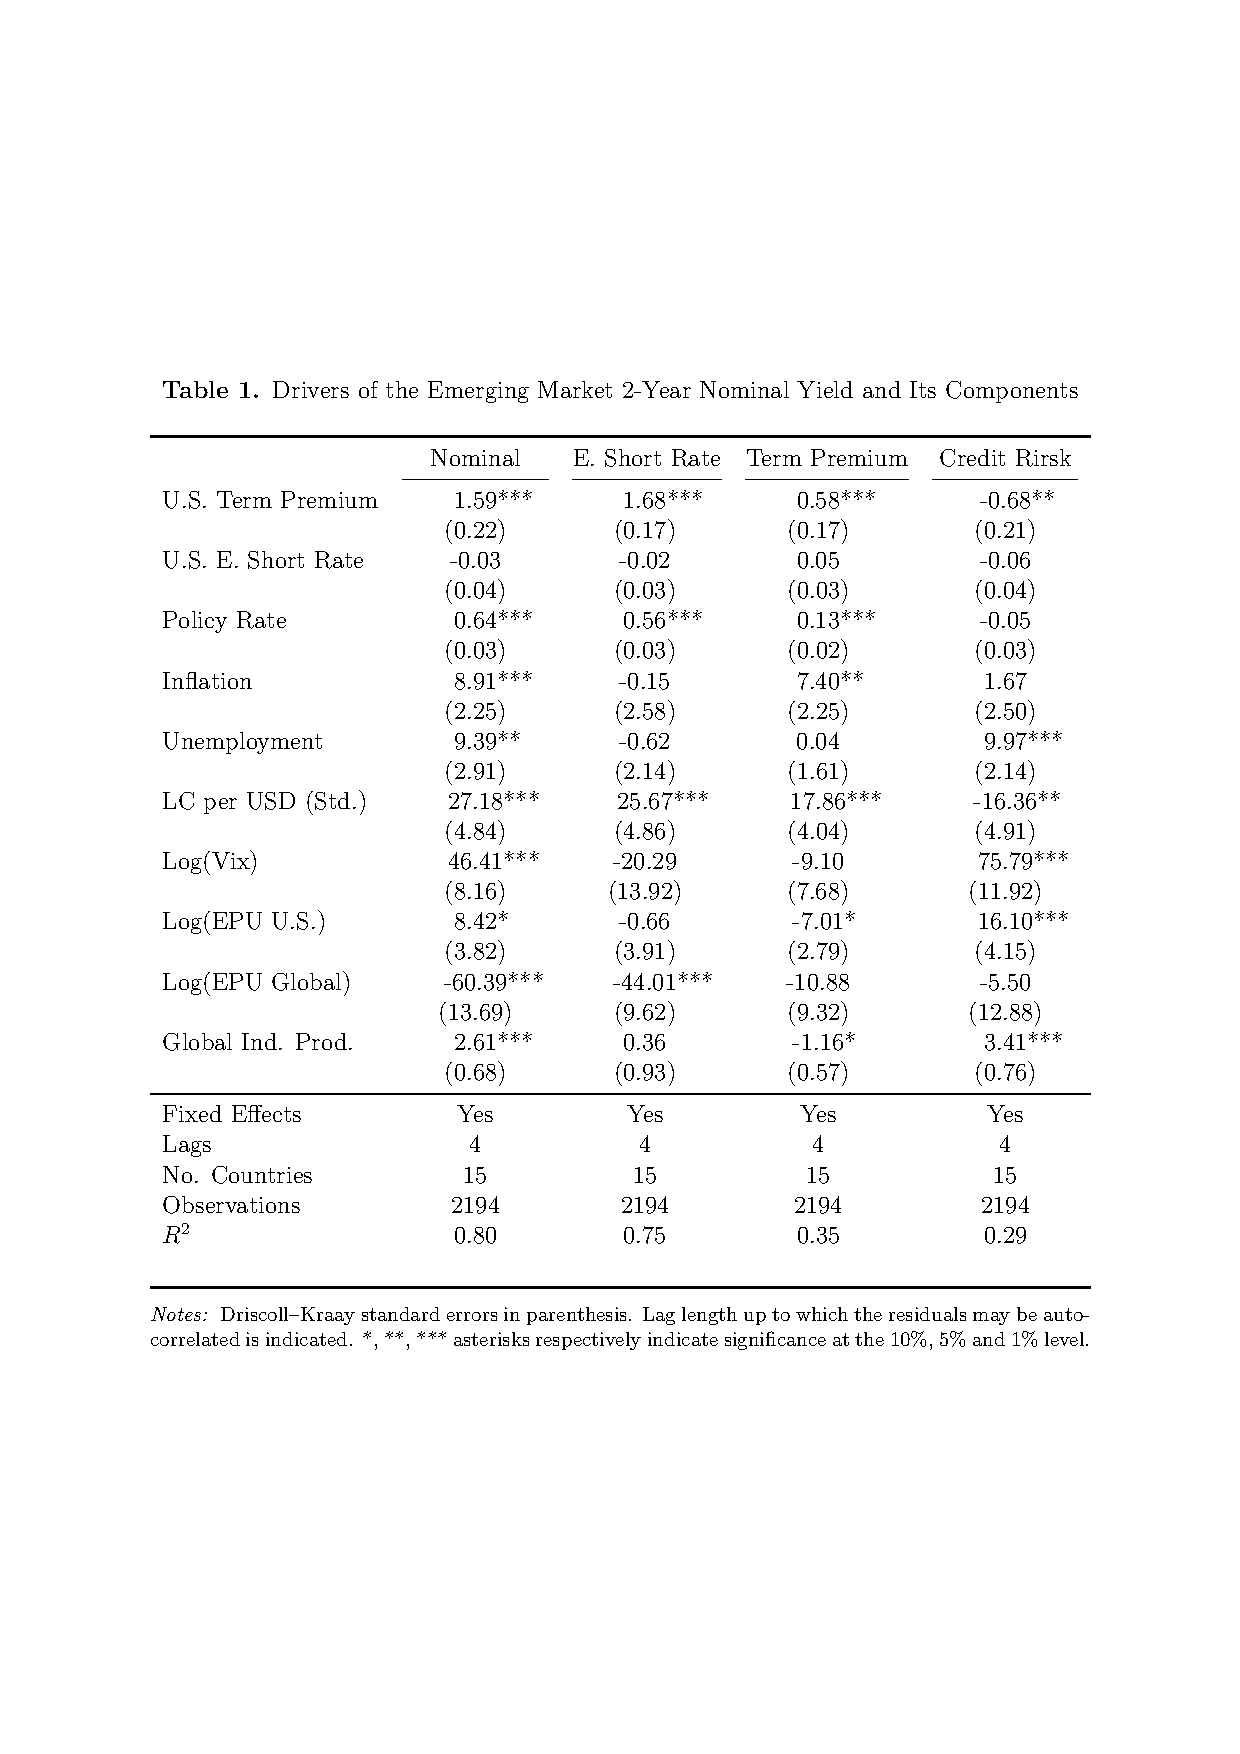
\includegraphics[trim={2cm 7.1cm 2cm 5cm},clip,height=1\textheight,width=0.85\textwidth]{../Tables/ycdcmp2y.pdf}};
%	%\draw[step=1cm,gray,very thin] (-4,-4) grid (6,6);
%	\draw[red,thick] (-6,1.6) rectangle (6,2.6);
%	\end{tikzpicture}
%\end{center}
%%\begin{figure}[!htbp]
%%	\begin{center} % trim removes: left, down, right, top
%%		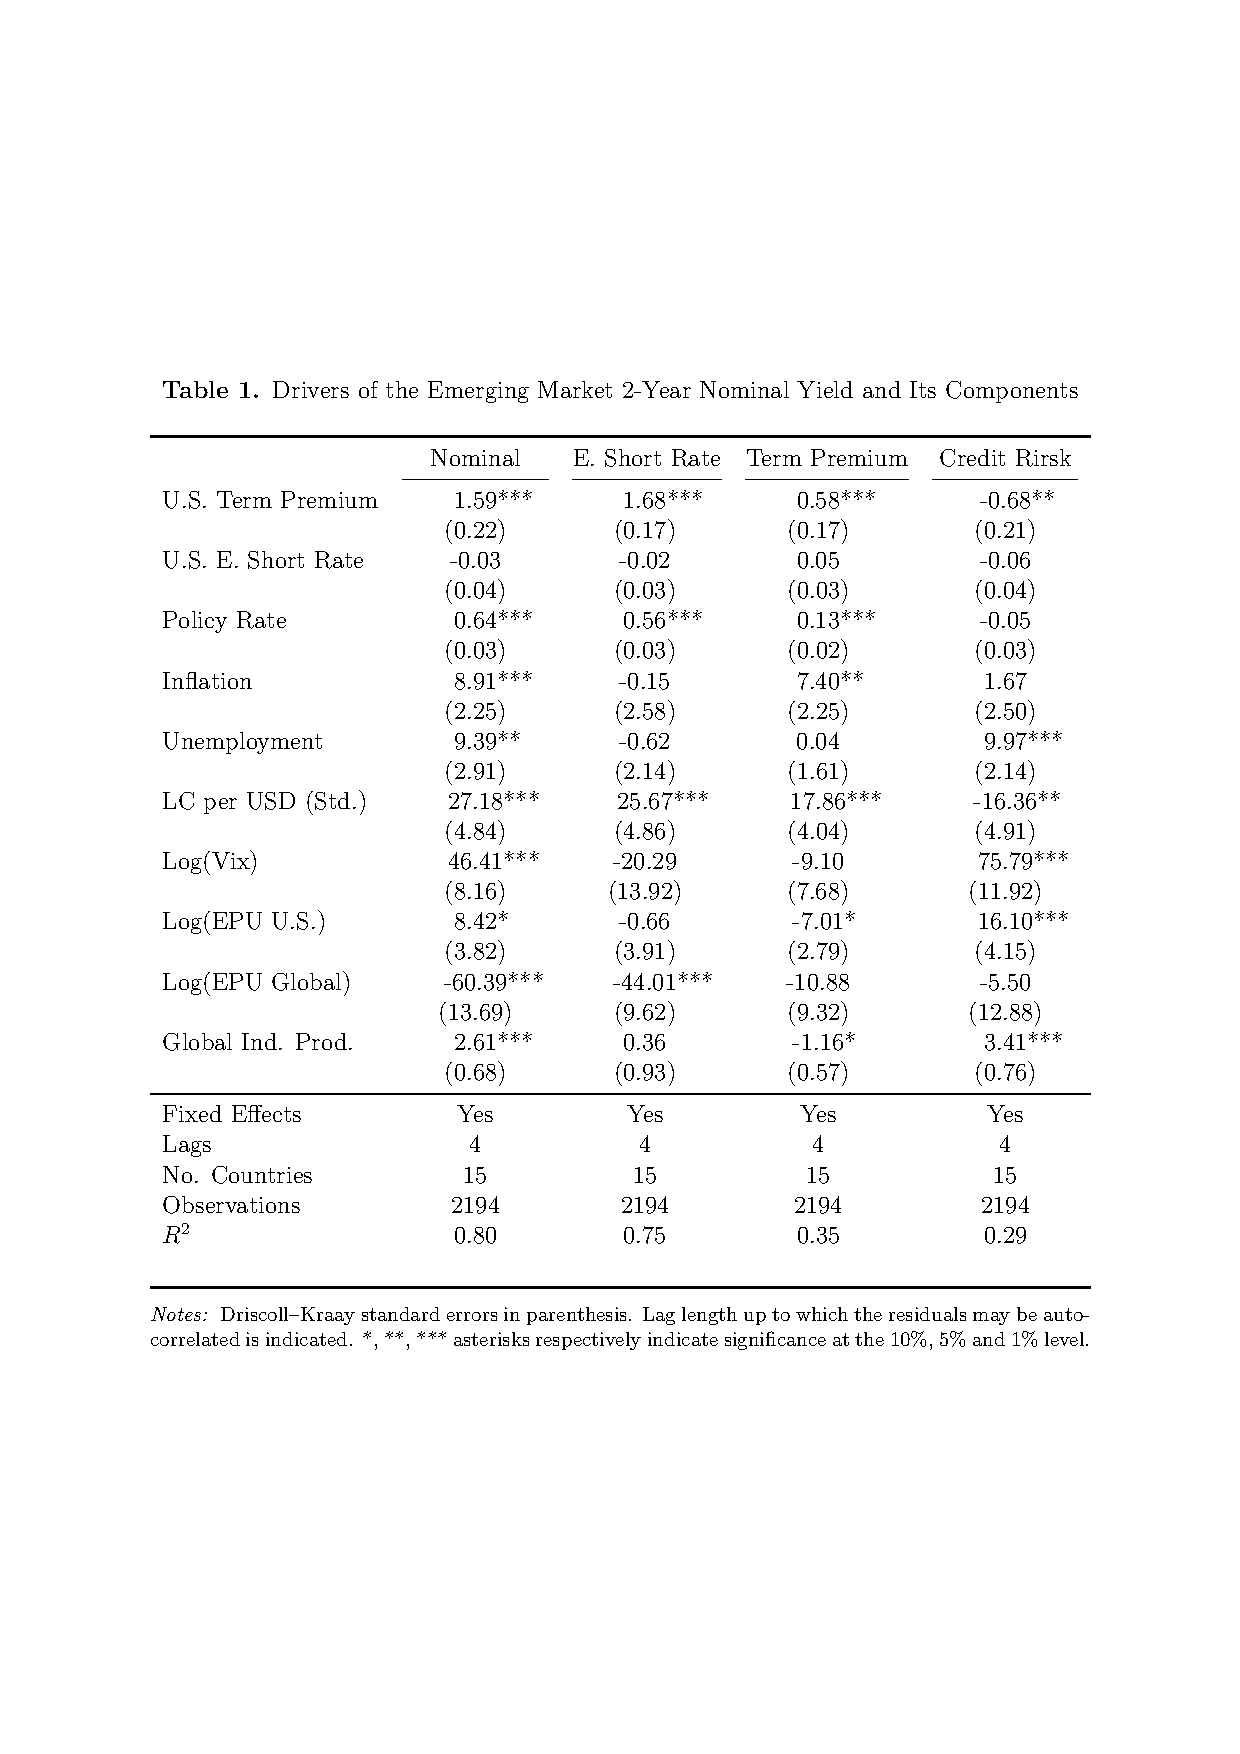
\includegraphics[trim={2cm 7.1cm 2cm 5cm},clip, width=0.85\textwidth,height=1\textheight]{../Tables/ycdcmp2y.pdf}
%%		\par\end{center}
%%\end{figure}
%\end{frame}
%
%\begin{frame}
%%	\frametitle{EM Term Premium and Inflation Uncertainty}
%\vspace{-0.8cm}
%\begin{center}
%	\begin{tikzpicture}
%	\node (table) at (0,0)
%	{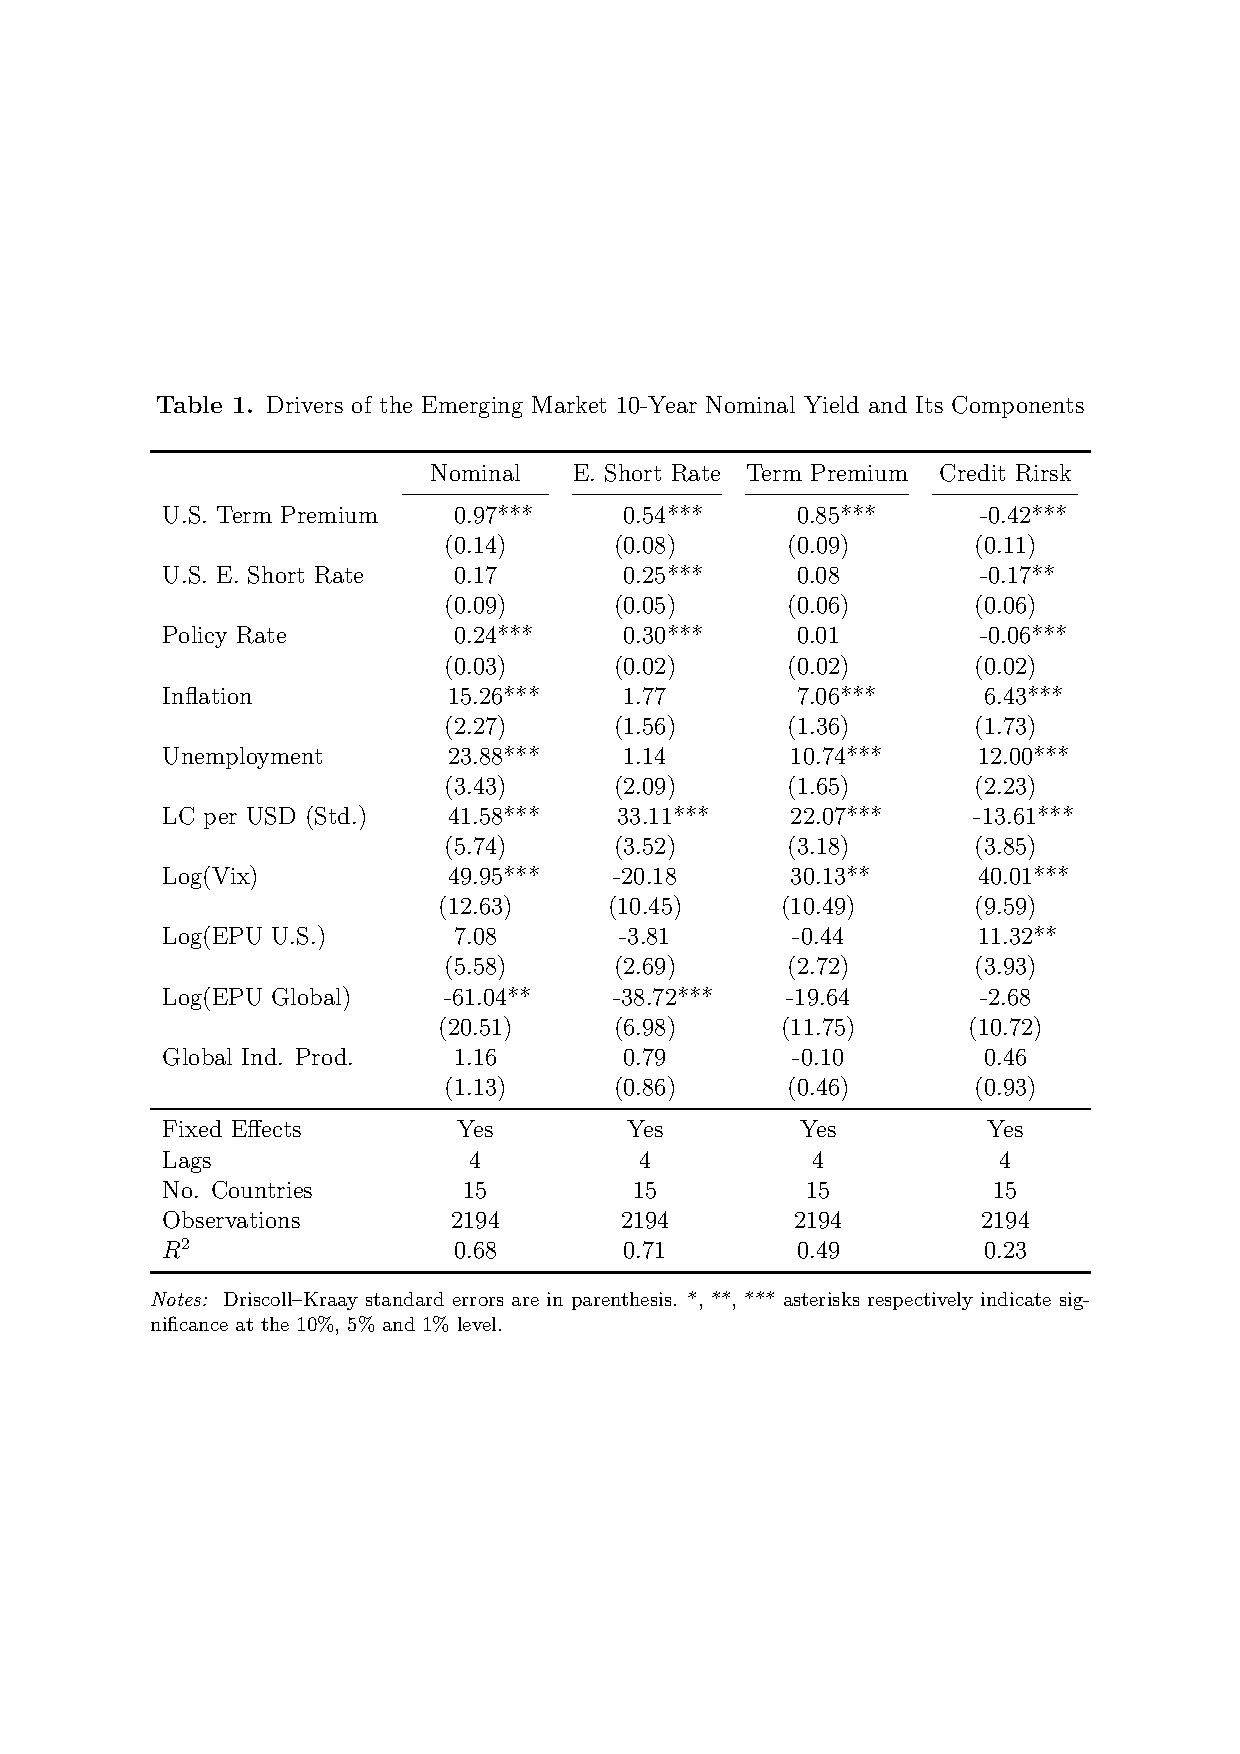
\includegraphics[trim={2cm 7.1cm 2cm 5cm},clip,height=1\textheight,width=0.85\textwidth]{../Tables/ycdcmp10y.pdf}};
%	%\draw[step=1cm,gray,very thin] (-4,-4) grid (6,6);
%	\draw[red,thick] (-6,1.6) rectangle (6,2.6);
%	\end{tikzpicture}
%\end{center}
%\end{frame}


\begin{frame}
\frametitle{U.S. Monetary Policy Surprises}
\begin{itemize}
	\item Asset price changes: 2-hour windows around FOMC meetings since 2000
	\item Surprises: \cite*{Kuttner:2001,GSS:2005a}
	\begin{itemize}
		\item Target (2000-2008): federal funds futures contracts
		\item Forward guidance (2000-2019): residual of ED8 yield on target surprise
		\item Asset purchase (2009-2019): residual of 10Y Treasury yield on target and forward guidance surprises
	\end{itemize}
\end{itemize}
\end{frame}

\begin{frame}
	\frametitle{U.S. Monetary Policy Effects on EM Yields}
	\vspace{-1cm}
	\begin{equation*} \label{eq:uPanelLP}
	\eqpanelLP
\end{equation*}	% \ref{eq:nPanelLP}
	\vspace{-0.7cm}
	\begin{itemize}
		\item \(\yld_{\idxspnl}\): 10- and 2-year nominal yields and their components
		\item \(\idxh\): horizon in days with \(\idxh = 0, 1, \ldots, 45\)
		\item \(\alpha_{\idxh,\idxi}\): country fixed effects
		\item \(\epsilon^{j}_{\idxt}\): three types of monetary policy surprises
		\item \(\fx_{\idxspnllag}\): one-day lag in the exchange rate
	\end{itemize}
\end{frame}
\note{Evidence of delayed response in AE.}
\note{All responses are assessed relative to a one basis point reduction (an easing) in any of the surprises.}
\note{DK SE, 90\% confidence bands}

\begin{frame}[label=TargetEM]
	\frametitle{Effects of Target Surprises}
	\begin{figure}[!htbp]
		\begin{center} % trim removes: left, down, right, top
			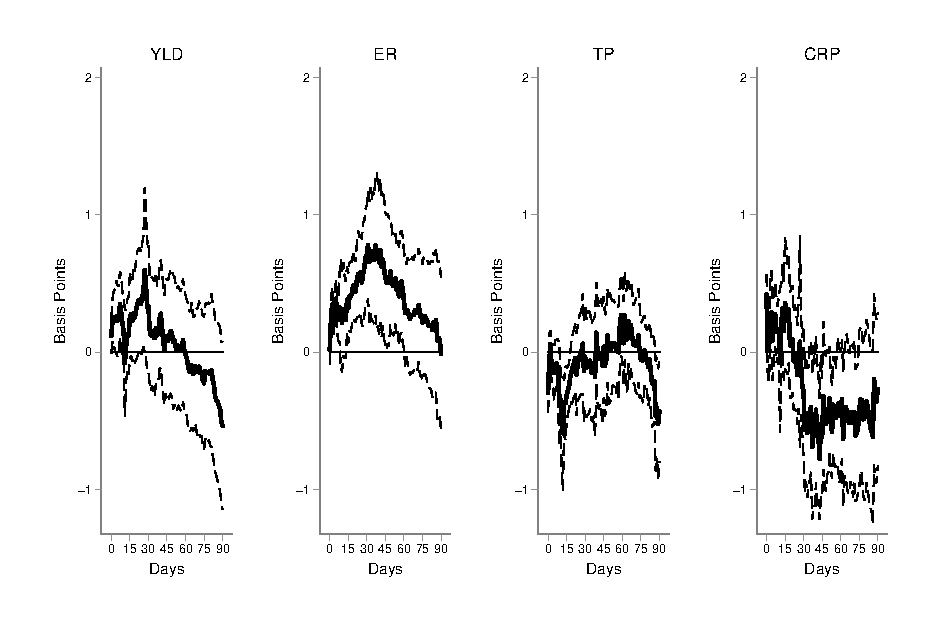
\includegraphics[trim={0cm 0cm 0cm 0cm},clip,height=0.4\textheight,width=0.85\linewidth]{../Figures/LPs/LagDep-FX/Target/EM/TargetEMnomyptpphi120m.eps}
			\par\end{center}
	\end{figure}
	\vspace{-0.5cm}
	\begin{figure}[!htbp]
		\begin{center} % trim removes: left, down, right, top
			\includegraphics[trim={0cm 0cm 0cm 0.76cm},clip,height=0.4\textheight,width=0.85\linewidth]{../Figures/LPs/LagDep-FX/Target/EM/TargetEMnomyptpphi24m.eps}
			\par\end{center}
	\end{figure}
	\begin{textblock*}{8mm}(10mm,34mm)
		\small 10Y
	\end{textblock*}
	\begin{textblock*}{8mm}(10mm,65mm)
		\small 2Y
	\end{textblock*}
\begin{textblock*}{5cm}(.95\textwidth,0.11\textheight)
	\hyperlink{TargetUS}{\beamergotobutton{US}}
\end{textblock*}
\end{frame}

\begin{frame}[label=FGEM]
	\frametitle{Effects of Forward Guidance Surprises}
	\begin{figure}[!htbp]
		\begin{center} % trim removes: left, down, right, top
			\includegraphics[trim={0cm 0cm 0cm 0cm},clip,height=0.4\textheight,width=0.85\linewidth]{../Figures/LPs/LagDep-FX/Path/EM/PathEMnomyptpphi120mPost.eps}
			\par\end{center}
	\end{figure}
	\vspace{-0.5cm}
	\begin{figure}[!htbp]
		\begin{center} % trim removes: left, down, right, top
			\includegraphics[trim={0cm 0cm 0cm 0.76cm},clip,height=0.4\textheight,width=0.85\linewidth]{../Figures/LPs/LagDep-FX/Path/EM/PathEMnomyptpphi24mPost.eps}
			\par\end{center}
	\end{figure}
	\begin{textblock*}{8mm}(10mm,34mm)
		\small 10Y
	\end{textblock*}
	\begin{textblock*}{8mm}(10mm,65mm)
		\small 2Y
	\end{textblock*}
	\begin{textblock*}{5cm}(.95\textwidth,0.11\textheight)
		\hyperlink{FGUS}{\beamergotobutton{US}}
	\end{textblock*}
\end{frame}

\begin{frame}[label=LSAPEM]
	\frametitle{Effects of Asset Purchase Surprises}
	\begin{figure}[!htbp]
		\begin{center} % trim removes: left, down, right, top
			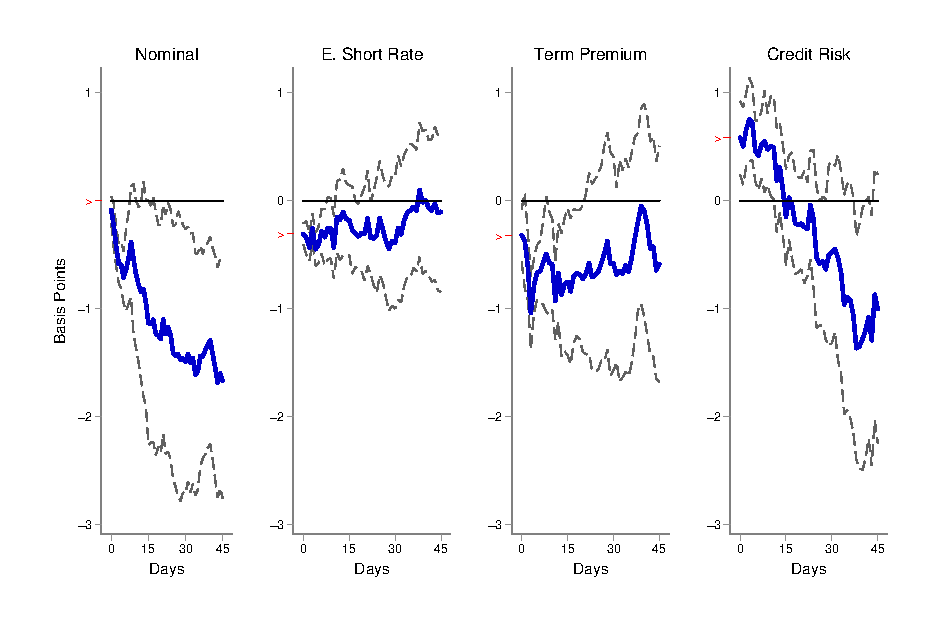
\includegraphics[trim={0cm 0cm 0cm 0cm},clip,height=0.4\textheight,width=0.85\linewidth]{../Figures/LPs/LagDep-FX/LSAP/EM/LSAPEMnomyptpphi120m.eps}
			\par\end{center}
	\end{figure}
	\vspace{-0.5cm}
	\begin{figure}[!htbp]
		\begin{center} % trim removes: left, down, right, top
			\includegraphics[trim={0cm 0cm 0cm 0.76cm},clip,height=0.4\textheight,width=0.85\linewidth]{../Figures/LPs/LagDep-FX/LSAP/EM/LSAPEMnomyptpphi24m.eps}
			\par\end{center}
	\end{figure}
	\begin{textblock*}{8mm}(10mm,34mm)
		\small 10Y
	\end{textblock*}
	\begin{textblock*}{8mm}(10mm,65mm)
		\small 2Y
	\end{textblock*}
	\begin{textblock*}{5cm}(.95\textwidth,0.11\textheight)
		\hyperlink{LSAPUS}{\beamergotobutton{US}}
	\end{textblock*}
\end{frame}

\section{Conclusions}

\begin{frame}
	\frametitle{Conclusions}
	\begin{itemize}
		\item Three-part decomposition of EM yields
		\begin{itemize}
			\item Average expected short rate, term premium, credit risk compensation
		\end{itemize}
		\item U.S. monetary policy spillovers
		\begin{enumerate}
			\item Responses are economically significant yet delayed
			\item Reassessment of policy rate expectations, repricing of risks
			\item Evidence of a yield curve channel since 2008
		\end{enumerate}
	\end{itemize}
\end{frame}
\note{YC channel: EM monetary autonomy decreases along the yield curve and involves the credit risk compensation.}
\note{To understand comovement, I propose a decomposition of EM yields.}
\note{Extensions: nominal-real decompositions, jumps.}


\section{Appendix}

\begin{frame}
	\begin{center}
		\huge \textcolor{yaleblue}{Appendix}
	\end{center}
\end{frame}


\begin{frame}[label=yPscbp]
%	\frametitle{Components: Expected Future Short Rate}
\begin{center}							% center the figure inside the minipage
	\includegraphics[trim={0cm 0cm 0cm 0cm},clip,height=0.86\textheight,width=\linewidth]{../Figures/Estimation/bsl_yP_scbp.eps} \\
\end{center}
\begin{textblock*}{5cm}(.89\textwidth,0.05\textheight)
	\hyperlink{YldDcmp}{\beamergotobutton{Decomposition}}
\end{textblock*}
\end{frame}

\begin{frame}[label=tpCI]
%	\frametitle{Components: Term Premium}
\begin{center}							% center the figure inside the minipage
\includegraphics[trim={0cm 0cm 0cm 0cm},clip,height=0.86\textheight,width=\linewidth]{../Figures/Estimation/bsl_tp_CI_10y_V1.eps} \\
\end{center}
\begin{textblock*}{5cm}(.89\textwidth,0.05\textheight)
	\hyperlink{YldDcmp}{\beamergotobutton{Decomposition}}
\end{textblock*}
\end{frame}
\note{Survey-Based Term Premium Estimates}
\note{EM TP are time-varying.}
\note{Sensible TP estimates, mostly positive; fluctuate between 0\% and 5\%.}
\note{Sometimes they comove.}

\begin{frame}[label=crcCI]
%\frametitle{Components: Credit Risk Compensation}
\begin{center}							% center the figure inside the minipage
	\includegraphics[trim={0cm 0cm 0cm 0cm},clip,height=0.86\textheight,width=\linewidth]{../Figures/Estimation/bsl_cr_CI_10y_V1.eps} \\
\end{center}
\begin{textblock*}{5cm}(.89\textwidth,0.05\textheight)
	\hyperlink{YldDcmp}{\beamergotobutton{Decomposition}}
\end{textblock*}
\end{frame}

\begin{frame}[label=TargetUS]
\frametitle{Effects of Target Surprises}
\begin{figure}[!htbp]
	\begin{center} % trim removes: left, down, right, top
		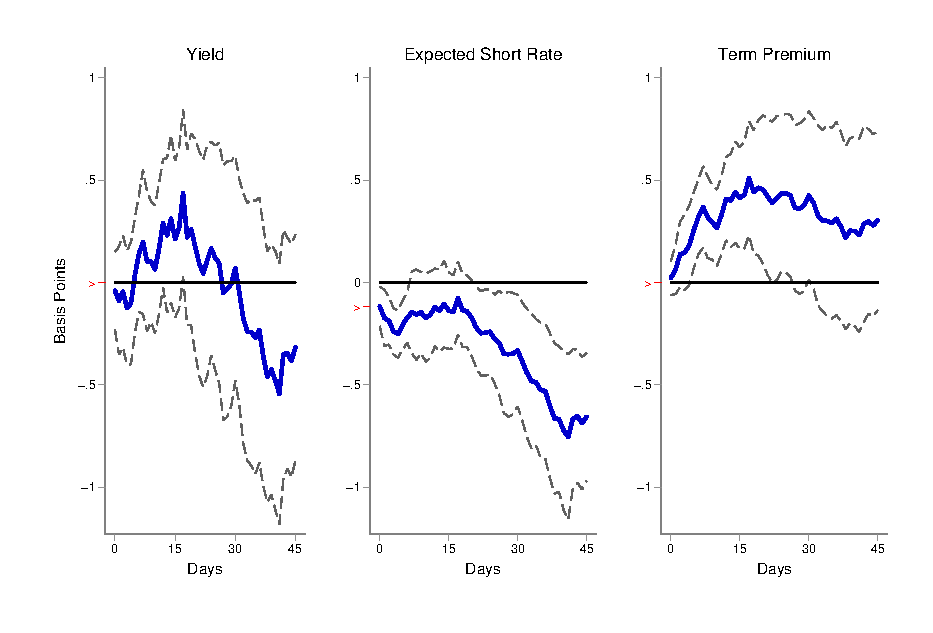
\includegraphics[trim={0cm 0cm 0cm 0cm},clip,height=0.4\textheight,width=0.85\linewidth]{../Figures/LPs/LagDep-FX/Target/US/DCMP/TargetUSDnomyptp120m.eps}
		\par\end{center}
\end{figure}
\vspace{-0.5cm}
\begin{figure}[!htbp]
	\begin{center} % trim removes: left, down, right, top
		\includegraphics[trim={0cm 0cm 0cm 0.76cm},clip,height=0.4\textheight,width=0.85\linewidth]{../Figures/LPs/LagDep-FX/Target/US/DCMP/TargetUSDnomyptp24m.eps}
		\par\end{center}
\end{figure}
\begin{textblock*}{8mm}(10mm,34mm)
	\small 10Y
\end{textblock*}
\begin{textblock*}{8mm}(10mm,65mm)
	\small 2Y
\end{textblock*}
\begin{textblock*}{5cm}(.95\textwidth,0.11\textheight)
	\hyperlink{TargetEM}{\beamergotobutton{EM}}
\end{textblock*}
\end{frame}

\begin{frame}[label=FGUS]
\frametitle{Effects of Forward Guidance Surprises}
\begin{figure}[!htbp]
\begin{center} % trim removes: left, down, right, top
	\includegraphics[trim={0cm 0cm 0cm 0cm},clip,height=0.4\textheight,width=0.85\linewidth]{../Figures/LPs/LagDep-FX/Path/US/DCMP/PathUSDnomyptp120mPost.eps}
	\par\end{center}
\end{figure}
\vspace{-0.5cm}
\begin{figure}[!htbp]
\begin{center} % trim removes: left, down, right, top
	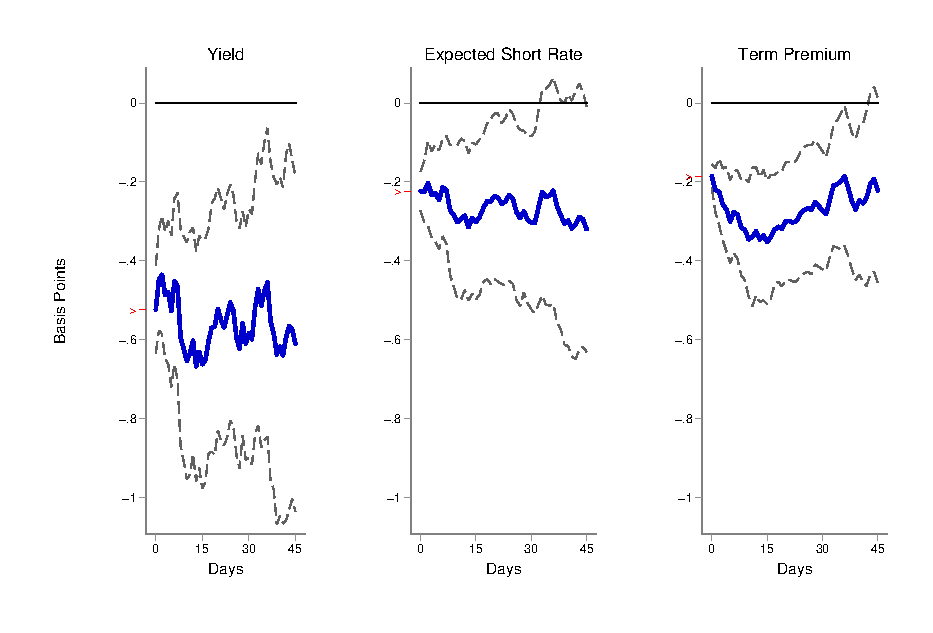
\includegraphics[trim={0cm 0cm 0cm 0.76cm},clip,height=0.4\textheight,width=0.85\linewidth]{../Figures/LPs/LagDep-FX/Path/US/DCMP/PathUSDnomyptp24mPost.eps}
	\par\end{center}
\end{figure}
\begin{textblock*}{8mm}(10mm,34mm)
\small 10Y
\end{textblock*}
\begin{textblock*}{8mm}(10mm,65mm)
\small 2Y
\end{textblock*}
\begin{textblock*}{5cm}(.95\textwidth,0.11\textheight)
	\hyperlink{FGEM}{\beamergotobutton{EM}}
\end{textblock*}
\end{frame}

\begin{frame}[label=LSAPUS]
\frametitle{Effects of Asset Purchase Surprises}
\begin{figure}[!htbp]
\begin{center} % trim removes: left, down, right, top
\includegraphics[trim={0cm 0cm 0cm 0cm},clip,height=0.4\textheight,width=0.85\linewidth]{../Figures/LPs/LagDep-FX/LSAP/US/DCMP/LSAPUSDnomyptp120m.eps}
\par\end{center}
\end{figure}
\vspace{-0.5cm}
\begin{figure}[!htbp]
\begin{center} % trim removes: left, down, right, top
\includegraphics[trim={0cm 0cm 0cm 0.76cm},clip,height=0.4\textheight,width=0.85\linewidth]{../Figures/LPs/LagDep-FX/LSAP/US/DCMP/LSAPUSDnomyptp24m.eps}
\par\end{center}
\end{figure}
\begin{textblock*}{8mm}(10mm,34mm)
\small 10Y
\end{textblock*}
\begin{textblock*}{8mm}(10mm,65mm)
\small 2Y
\end{textblock*}
\begin{textblock*}{5cm}(.95\textwidth,0.11\textheight)
	\hyperlink{LSAPEM}{\beamergotobutton{EM}}
\end{textblock*}
\end{frame}


\begin{frame}<presentation:0>
\bibliographystyle{abbrvnat} 
\bibliography{../../../References/library}
\end{frame}

\end{document}

%---------------------------------------------------------------
% Sources
%---------------------------------------------------------------
% Tips in general
% https://en.wikibooks.org/wiki/LaTeX/Presentations
%https://tex.stackexchange.com/questions/12328/how-can-i-use-todonotes-with-beamer
% Insert links to slides
% https://latex.org/forum/viewtopic.php?t=4594
% Place button of link on slide
%https://tex.stackexchange.com/questions/50643/hyperlink-button-in-an-exact-position
% Make figures visible
%https://stackoverflow.com/questions/4683093/beamer-how-to-show-images-as-step-by-step-images
% Multicolumn and multirow
%https://tex.stackexchange.com/questions/156219/proper-centering-with-cmidrule-and-multi-row-and-column

% Code for hyperlinks
%[label=corr_10yr]
%\begin{textblock*}{3cm}(.9\textwidth,-.5\textheight)
%	\hyperlink{corr_10yr}{\beamergotobutton{10-Year TP}}
%\end{textblock*}
%
%\begin{textblock*}{3cm}(.9\textwidth,-.5\textheight)
%	\hyperlink{corr_10yr}{\beamerreturnbutton{10-Year TP}}
%\end{textblock*}

% Two-column frame template
%http://felix11h.github.io/blog/beamer-two-col


%---------------------------------------------------------------
% Previous versions
%---------------------------------------------------------------
% \begin{frame}
%	\frametitle{Motivation}
%	\begin{itemize}
%		\item \textit{Risk-free} zero-coupon yields can be decomposed into: 
%		\begin{itemize}
%			\item Expected short-term interest rate
%			\item Term premium
%		\end{itemize}
%		\iftoggle{struct}{\item<2->}{\item} Sovereign debt of advanced economies is considered risk-free
%		\iftoggle{struct}{\item<3>}{\item} \textbf{Problem:} Debt of emerging markets (EMs) is \textit{not} risk-free
%		\begin{itemize}
%		\iftoggle{struct}{\item<3>}{\item} Credit risks embedded in local currency (LC) debt
%		\end{itemize}
%		% \textcolor{yaleblue}{\textbf{Gap:}}	% To color text
%	\end{itemize}
%\end{frame}
%\note{Term premium: Compensation that investors require for bearing the risk that the short-term yield does not evolve as they expected. If LT bonds are seen as risky, need compensation so RP > 0; if they are seen as a hedge, investors are willing to receive less than what is expected for the short term rate and so RP < 0.}
%\note{Sometimes TP is used interchangably with RP. I will use TP.}
%\note{Credit risk understood as: (selective) default risk, currency convertibility risk, regulation risk, capital controls, jurisdiction risks, liquidity risk.}
%\note{Why default on LC debt? FC debt creates trade-off between default and inflating away LC; small cost to default in LC if already defaulted on FC; EMs can change the law + Suspension of currency convertibility, capital controls while not defaulting.}
%\note{The questions is: how can we decompose LC yield curves in EMs? What can we learn by taking into accout these risks?}
%
%\begin{frame}
%	\frametitle{What Do I Do?}
%	\begin{itemize}
%		\item Decompose LC yields of EMs \textit{without} credit risk
%		\begin{itemize}
%			\item Analyze components, especially the term premium
%		\end{itemize}
%		\iftoggle{long}{\pause}{}
%		\item \textbf{Main idea:} What if the U.S. issue debt in other currencies?
%		\iftoggle{long}{\pause}{}
%		\begin{itemize}
%			\item Use synthetic zero-coupon yield curves
%			\item Swap U.S. Treasury yields into LC using derivatives
%			\begin{itemize}
%				\item Forward premium
%			\end{itemize}
%		\end{itemize}
%	\end{itemize}
%\end{frame}
%\note{Today I can lock in a risk-free investment in LC by exchanging LC for USD, investing those USD in Tresuaries and enter into a forward agreeing to sell USD for LC in the future. Once I receive the payment from Treasuries, I exchange them into LC.}
%
%\begin{frame}
%	\frametitle{Why Is This Important?}
%	\begin{itemize}
%		\item Determinants of LC yields
%		\begin{itemize}
%			\item Market expectations about monetary policy
%			\item Monetary policy transmission in EMs
%		\end{itemize}
%		\iftoggle{struct}{\item<2->}{\item} Global financial cycle
%		\begin{itemize}
%			\iftoggle{struct}{\item<2->}{\item} EMs vs advanced economies
%		\end{itemize}
%		\iftoggle{struct}{\item<3>}{\item} Testing asset pricing theories in EMs
%		\begin{itemize}
%			\iftoggle{struct}{\item<3>}{\item} Buraschi, Piatti and Whelan (2018)
%		\end{itemize}
%	\end{itemize}
%\end{frame}
%\note{The analysis opens the door to interesting research!!!}
%\note{Use proxies of the determinants of term premia implied by equilibrium models.}
%\note{Risk premia is affected by disagreement (interquartile range in GDP and CPI forecasts), habit preferences (monthly consumption growth rates), uncertainty of conditional growth rate (conditional variance of expected real growth and inflation).}
%
%\begin{frame}
%	\frametitle{What Has Been Done?}
%	\begin{itemize}
%		\item Vast literature on yield curve decomposition for advanced economies (AEs)
%		\item Fewer papers decompose of EM yield curves
%		\begin{itemize}
%			\item \citet*{BlakeRuleRummel:2015}
%		\end{itemize}
%		\iftoggle{struct}{\item<2->}{\item} Synthetic yield curves
%		\begin{itemize}
%			\iftoggle{struct}{\item<2->}{\item} LC credit spread \citep{DuSchreger:2016a}
%			\iftoggle{struct}{\item<2->}{\item} Convenience yield \citep*{DuImSchreger:2018}
%		\end{itemize}
%	\end{itemize}
%\end{frame}
%\note{Du \& Schreger (2016) developed an empirical measure to assess credit risk in LC debt.}

%\begin{frame}
%\frametitle{Credit Risk in EM Yields}
%\begin{itemize}
%	\item \textit{Credit-risk-free} yields reflect: 
%	\begin{itemize}
%		\item Expected short-term interest rate
%		\item Term premium
%	\end{itemize}
%\end{itemize}
%\end{frame}
%\note{Term premium: Compensation for bearing interest rate risk, locking your money instead of rolling it over.}
%\note{Broad perspective on credit risk, i.e. not receiving promised payments: EMs can change the law + Suspension of currency convertibility + Capital controls + Actual default.}
%\note{Sovereign debt of AEs is considered free of credit risk.}
%\note{Synthetic instead of nominal yields.}
%\note{US YC used as a benchmark for all EMs.}
%\note{FX forwards and XCS used to get the forward premium are collateralized.}
%\note{Today I can lock in a risk-free investment in LC by exchanging LC for USD, investing those USD in Tresuaries and enter into a forward agreeing to sell USD for LC in the future. Once I receive the payment from Treasuries, I exchange them into LC.}

%\begin{frame}
%	\frametitle{Affine Term Structure Model}
%	\begin{itemize}
%		\item ATSM standard tool to estimate dynamics of \textit{risk-free} \alert{nominal} yield curves
%		\begin{itemize}
%			\item A set of pricing factors drives the dynamics of the term structure
%			\item No-arbitrage restrictions: Consistency in (cross section/time series) bond yields
%			\item Yields are affine functions of the pricing factors
%		\end{itemize}
%		\item Decomposition of risk-free nominal yields:
%		\begin{itemize}
%			\item Expected short-term interest rate
%			\item Term premium
%		\end{itemize}
%		\item Key assumption: Zero credit risk
%	\end{itemize}
%\end{frame}
%\note{The coefficients are functions of the maturity of the bond and the coefficients that determine the stochastic processes that drive the state variables.}
%\note{Once the parameters of the model are estimated, they can be used to estimate the term premium.}

%		\item To assess the relevance of the results:
%		\begin{itemize}
%			\item Compare estimated term premia of EMs to those of advanced SOEs
%			\item Compare the term premia obtained from both $\yLCnom$ and $\yLCsynt$
%		\end{itemize}

%\begin{frame}
%	\frametitle{Term Premia: Does It Matter Which Curve Is Used?}
%	\begin{tiny}\begin{table}\centering\begin{tabular}{l|cc}\toprule & Nominal & Synthetic \\\midrule EM & 2.17 & 1.74 \\A-SOE & 2.03 & 1.97 \\G-3 & 1.70 & 1.60 \\\bottomrule\end{tabular}\caption{10-Year Term Premium Comparison (\%).}\label{tab:tp_compare10yr}\end{table}\end{tiny}
%	\begin{itemize}
%		\item Difference between the two TP estimates is larger for EMs on average
%		\begin{itemize}
%			\item Null of equal means is rejected at $5$\% for 13 EMs vs 4 AEs
%			\item For EMs, risk premium $\neq$ term premium
%		\end{itemize}
%	\end{itemize}
%\end{frame}
%\note{The null of equal means is rejected at the $5$\% significance level for all EMs except Hungary and Malaysia. However, the null is only rejected for four AEs (Australia, Denmark, Japan and New Zealand).}

%\begin{frame}
%	\frametitle{Relationship with Risk and Uncertainty Measures}
%	\begin{itemize}
%		\item Comparison with US term premium
%		\begin{itemize}
%			\item TP
%			\item $\perp$TP
%		\end{itemize}
%		\item CIP deviations: 
%		\begin{itemize}
%			\item LC credit spread \citep{DuSchreger:2016a}
%			\item Convenience yield \citep{DuImSchreger:2018}
%		\end{itemize}
%		\item Uncertainty indexes \citep{BakerBloomDavis:2016}
%	\end{itemize}
%\end{frame}
%\note{EPU index is based on frequency of key words -economy, uncertainty, Fed- in newspapers. Only available for 5 countries in the sample.}

% Conclusions
%		\item `Clean' EM TP estimates using synthetic LC yield curves
%		\begin{itemize}
%			\item Gains from `adjusting' for credit risk
%			\item In EMs, risk premium $\neq$ term premium
%			\item More disaggregated decomposition of nominal LC yield curves
%		\end{itemize}
%		\item Properties of EM term premia
%		\item Several potential extensions

%\begin{frame}
%\frametitle{Survey-Based Term Premium Estimates}
%	\begin{figure}[!htbp]
		\begin{centering}
			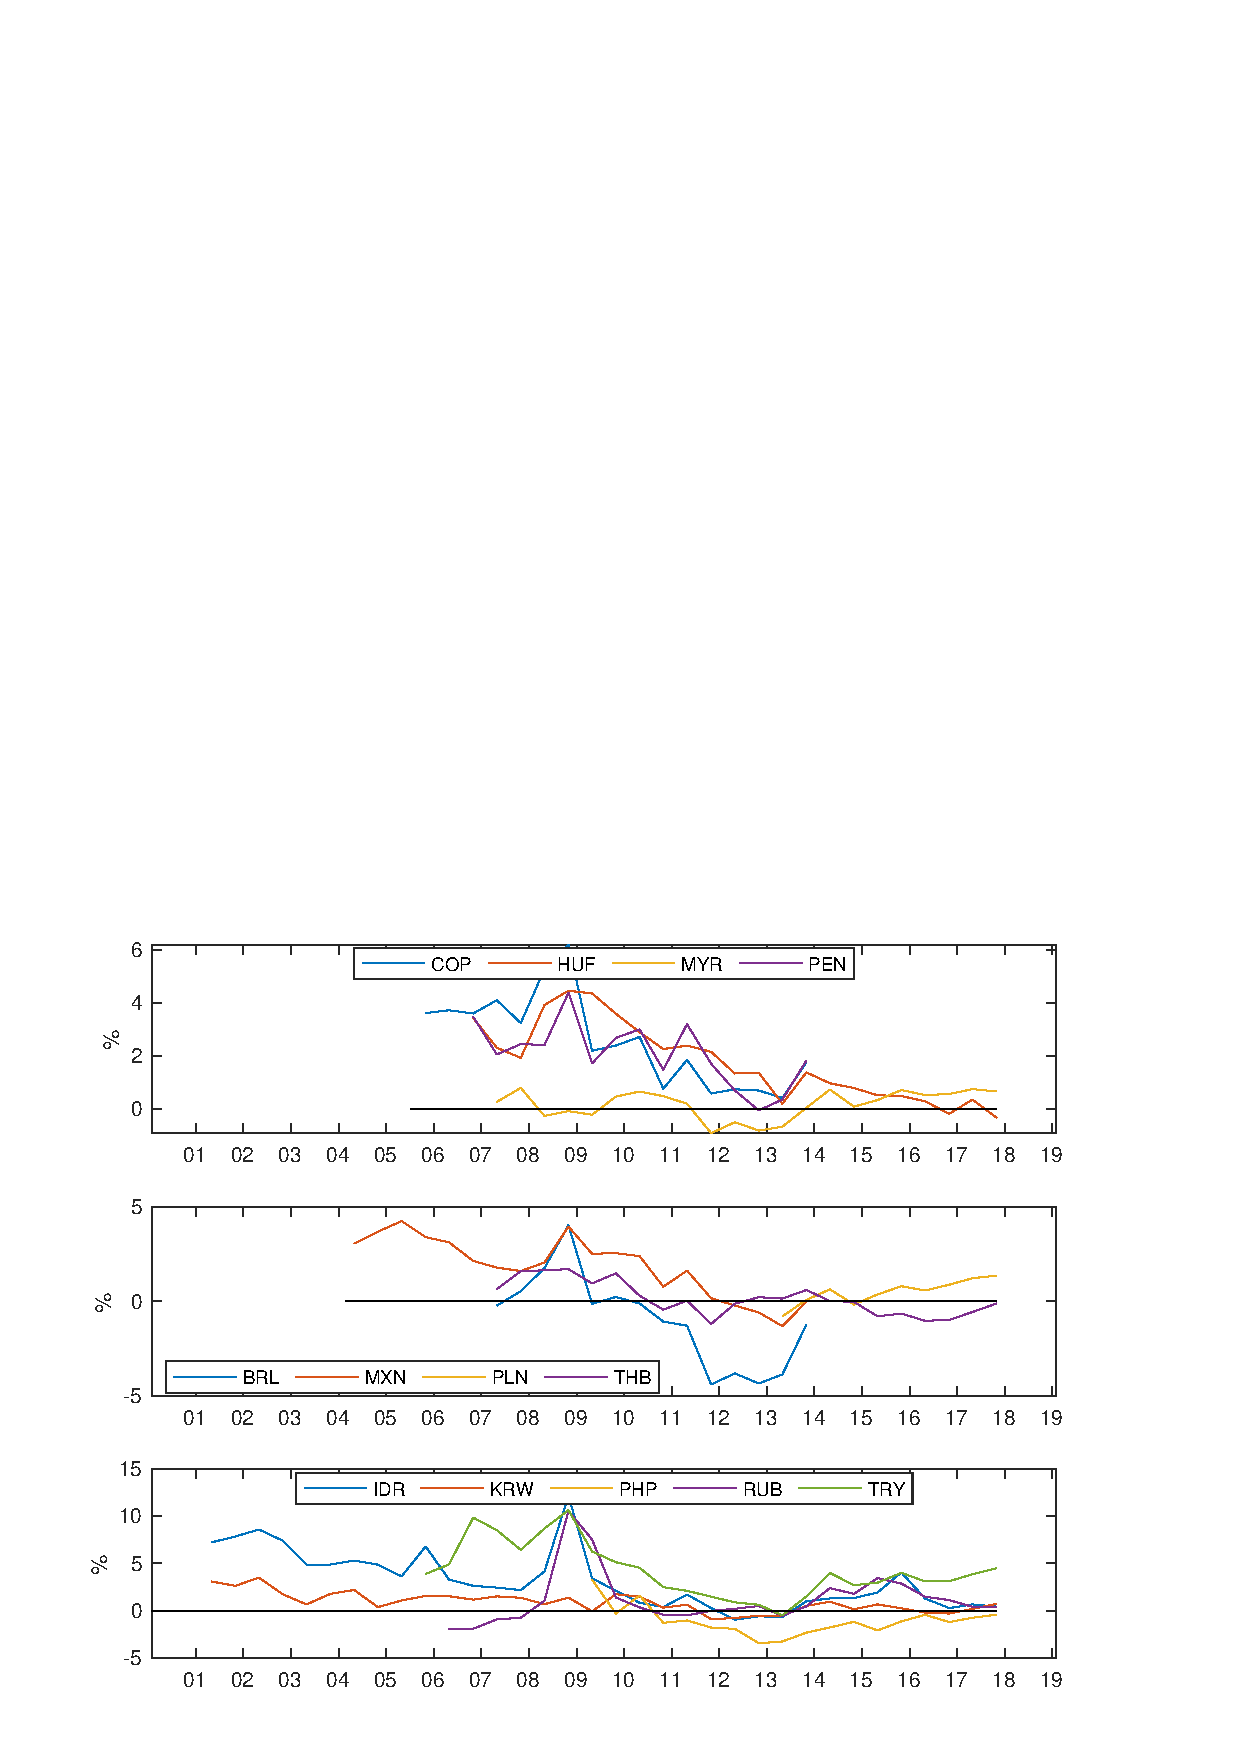
\includegraphics[width=1\textwidth,height=0.5\textheight]{../Figures/Temp/temp_tp10yrSvy}
			\par\end{centering}
		\caption{Survey-Based 10-Year Term Premium Estimates}\label{fig:temp_tp10yrSvy}
	\end{figure}
%%	\begin{textblock*}{3cm}(.97\textwidth,-.08\textheight)
%%		\hyperlink{tp_10yrA}{\beamerreturnbutton{A}}
%%	\end{textblock*}
%\end{frame}